% ------------------------------------------------------------------------------
% Mathematics Project Report Template
% by Jon Shiach 2019
% Manchester Metropolitan University
% ------------------------------------------------------------------------------
\documentclass[11pt]{report} 
\let\cleardoublepage\clearpage

% \cleardoubleoddpage
\usepackage{projectreport}
\usepackage{tikz}
\usetikzlibrary{shapes, arrows, positioning}
% ------------------------------------------------------------------------------
% Enter your details here
% ------------------------------------------------------------------------------
\usepackage{xcolor}  
% \usepackage{Arial}
% \usepackage[T1]{fontenc}
% \usepackage{mathptmx}
\newcommand{\name}{Mahmoud Essam Fathy 191900203\\[6pt]Hader Farag 191900162\\[6pt]Mariem Kamel 191900053\\[6pt]Alaa Kamal 191900057\\[6pt]}
\newcommand{\course}{Software maintenance and evaluation
 Project Report}
% \newcommand{\course}{BSc. (Hons) Financial Mathematics}
% \newcommand{\course}{MMath. (Hons) Mathematics}
% \newcommand{\course}{BSc. (Hons) Secondary Mathematics Education with QTS}
\newcommand{\projecttitle}{Wanas}
\newcommand{\submissiondate}{February 2024}
\usepackage{svg}

% ------------------------------------------------------------------------------
% Document
% ------------------------------------------------------------------------------
\begin{document}



    \maketitle

% ------------------------------------------------------------------------------
% Top matter
% ------------------------------------------------------------------------------
% \chapter*{Abstract}
% This graduation project delves into the realm of mental health support by introducing an innovative application designed to act as a virtual therapist. In a world where the pace of life is relentless and mental well-being is of paramount importance, our project aims to leverage artificial intelligence and machine learning to provide accessible and personalized assistance. The virtual therapist application offers users a confidential and empathetic space to express their thoughts and emotions, fostering a sense of connection and understanding. This documentation explores the design principles, underlying technologies, and ethical considerations that guided the development of the application. Additionally, it delves into the potential impact of such a solution on mental health care, addressing the pressing need for accessible and stigma-free support in today's digital landscape. Join us on this journey as we navigate the intersection of technology and mental health, contributing to the ongoing dialogue about innovative solutions for well-being in the modern age.
%
% \chapter*{Acknowledgements}
% We express deep gratitude for the collective support and contributions received during the completion of the graduation project. Special thanks are extended to academic mentors, advisors, peers, friends, family, participants, and the technological community. The acknowledgment emphasizes the collaborative nature of the project, recognizing the guidance, inspiration, and resources provided by various individuals and entities. It concludes with a sincere appreciation for everyone who played a role in the project's success and contributed to the academic and professional growth of the individuals involved.
% Wanas team\\
% ECU\\
% 2023
\tableofcontents 
% \listoffigures
% \listoftables
% \lstlistoflistings		% comment out if not needed

% ------------------------------------------------------------------------------
% Main matter
% Chapters are added to the document using the \include{chapterx} command
% ------------------------------------------------------------------------------
\newpage
\setcounter{page}{0}
\pagenumbering{arabic}
 ------------------------------------------------------------------------------
% Chapter 1
% ------------------------------------------------------------------------------
\chapter{Introduction}

\section{Brainstorming and Idea Development}

\subsection{Initial Brainstorming Sessions}
As part of the WANAS project launch, numerous brainstorming sessions were held to generate innovative approaches to providing mental health care. Our group convened to discuss several concepts and determine the most effective strategy. These sessions were crucial in shaping the initial concept of WANAS, ensuring that every idea was considered and discussed.

\subsection{Decision-Making Process}
After generating a wide array of ideas, the next step was to evaluate them. The team assessed each idea based on several key criteria:
\begin{itemize}
    \item \textbf{Feasibility:} Considering the practicality of implementing the idea within our available resources and timeframe.
    \item \textbf{Impact:} Evaluating how effectively the idea could address mental health needs and provide support to users.
    \item \textbf{Innovation:} Looking for unique and creative approaches that could set WANAS apart from other mental health support tools.
\end{itemize}
Through this structured decision-making process, we were able to narrow down our ideas and focus on the most promising concepts, laying a solid foundation for the development of WANAS.

\section{Inspiration Behind WANAS}
WANAS, named after the Arabic word  brings the comforting essence of companionship and joy to the digital realm. In Egyptian culture, represents the warmth and comfort of being with loved ones, feeling understood and supported. Our application embodies this spirit, offering users a virtual therapist that provides empathetic, personalized mental health support, ensuring that no one feels alone in their journey towards better mental health.

\section{Introduction to WANAS}

\subsection{Project Overview}
WANAS is a virtual therapist application designed to provide personalized mental health support. Utilizing advanced artificial intelligence and machine learning, WANAS aims to deliver empathetic, context-aware interactions through a user-friendly interface. The application prioritizes user privacy and data security, ensuring a safe environment for users to express their thoughts and emotions.

\subsection{Purpose and Motivation}

\subsubsection{Market Needs}
The WANAS application aims to fill critical gaps in the current mental health care landscape. Despite this high prevalence, traditional mental health services often struggle with issues like accessibility, affordability, and stigma. In many areas, especially in low- and middle-income countries, there is a significant shortage of mental health professionals, which makes it challenging for individuals to get timely and adequate care. The growing need for mental health support, along with the shortcomings of existing services, highlights the necessity for innovative solutions like a virtual therapist application.

\subsubsection{Academic Needs}
From an academic perspective, the project aligns with the growing interest in leveraging artificial intelligence and machine learning for healthcare applications. It provides a practical implementation of AI and ML techniques in a socially impactful domain. The project offers a rich case study for exploring ethical considerations in AI, user interaction design, and the development of adaptive systems. It also contributes to the body of research on digital mental health interventions, offering insights into their efficacy and user engagement.

\section{Understanding the Mental Health Crisis}

\subsection{Scope of the Problem}
Mental health issues are pervasive and affect people across all demographics worldwide. According to the World Health Organization (WHO), approximately 1 in 4 people will experience a mental health disorder at some point in their lives. This high prevalence reflects a wide range of conditions, from anxiety and depression to severe disorders like schizophrenia and bipolar disorder. Despite the widespread occurrence, there are significant challenges in addressing these issues effectively:
\begin{enumerate}
    \item \textbf{Accessibility:} Many regions, particularly low- and middle-income countries, face a severe shortage of mental health professionals. This shortage makes it difficult for individuals to receive timely and adequate care.
    \item \textbf{Affordability:} Traditional mental health services can be costly, making them inaccessible to large segments of the population, especially in regions without sufficient health insurance coverage or governmental support.
    \item \textbf{Stigma:} Social stigma surrounding mental health issues often prevents individuals from seeking help. Fear of judgment and discrimination can lead to reluctance in accessing mental health services.
    \item \textbf{Geographical Barriers:} In rural and remote areas, the availability of mental health services is often limited, requiring individuals to travel long distances to receive care.
    \item \textbf{Timeliness:} Traditional mental health services typically involve scheduled appointments, which may not be available immediately when individuals are in crisis.
\end{enumerate}

\subsection{Consequences of Untreated Mental Health Issues}
Untreated mental health issues have profound and multifaceted consequences, affecting individuals, families, communities, and society:
\begin{itemize}
    \item \textbf{Deterioration of Mental Health:} Symptoms can worsen over time, complicating daily life management.
    \item \textbf{Physical Health Problems:} Mental health issues can exacerbate chronic diseases and lead to unhealthy behaviors like substance abuse.
    \item \textbf{Decreased Quality of Life:} Affected individuals often struggle with relationships, employment, and enjoying activities.
    \item \textbf{Increased Risk of Suicide:} Conditions like depression and anxiety significantly heighten the risk of suicide.
    \item \textbf{Economic Impact:} Lost productivity, higher healthcare costs, and financial burdens on families and communities.
    \item \textbf{Social Consequences:} Stigma and isolation can result in social withdrawal and strained relationships.
    \item \textbf{Impact on Families and Communities:} Emotional distress, financial strain, and the challenge of providing support.
\end{itemize}


\begin{figure}[h]
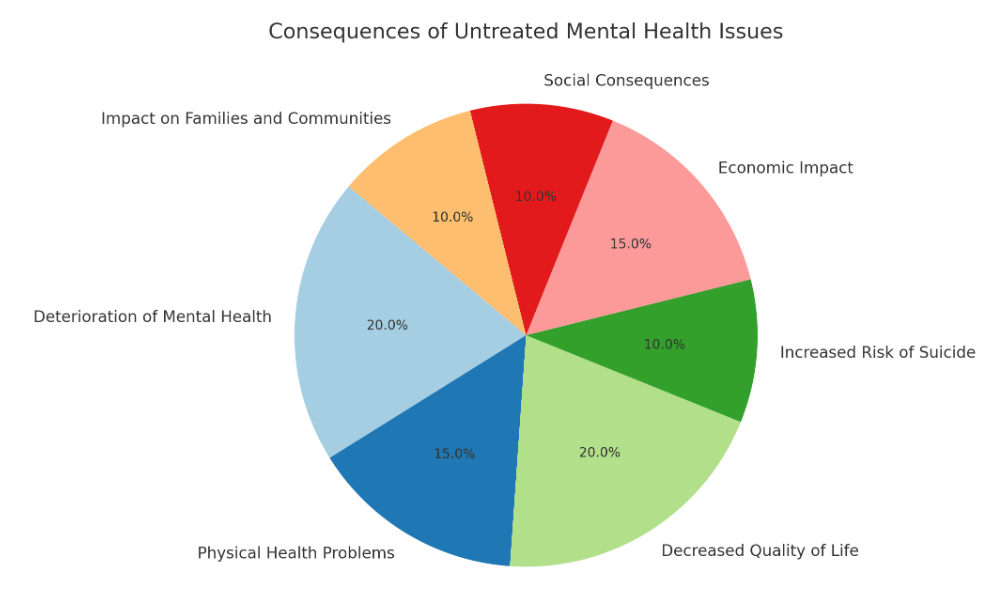
\includegraphics[width=\columnwidth]{intro}
\centering
\end{figure}

 ------------------------------------------------------------------------------
% Chapter 2
% ------------------------------------------------------------------------------
\chapter{Introduction} % enter the name of the chapter here
\section{ProjectIdea} % enter the name of the section here
\subsection{why?} %enter the name of the subsection here

 
 ------------------------------------------------------------------------------
% Chapter 1
% ------------------------------------------------------------------------------
\chapter{Analysis and Design} % enter the name of the chapter here
\cleardoublepage{}
\section{Diagrams} % enter the name of the section here

\subsection{Activity Diagram}
\begin{figure}[h]
    \begin{center}
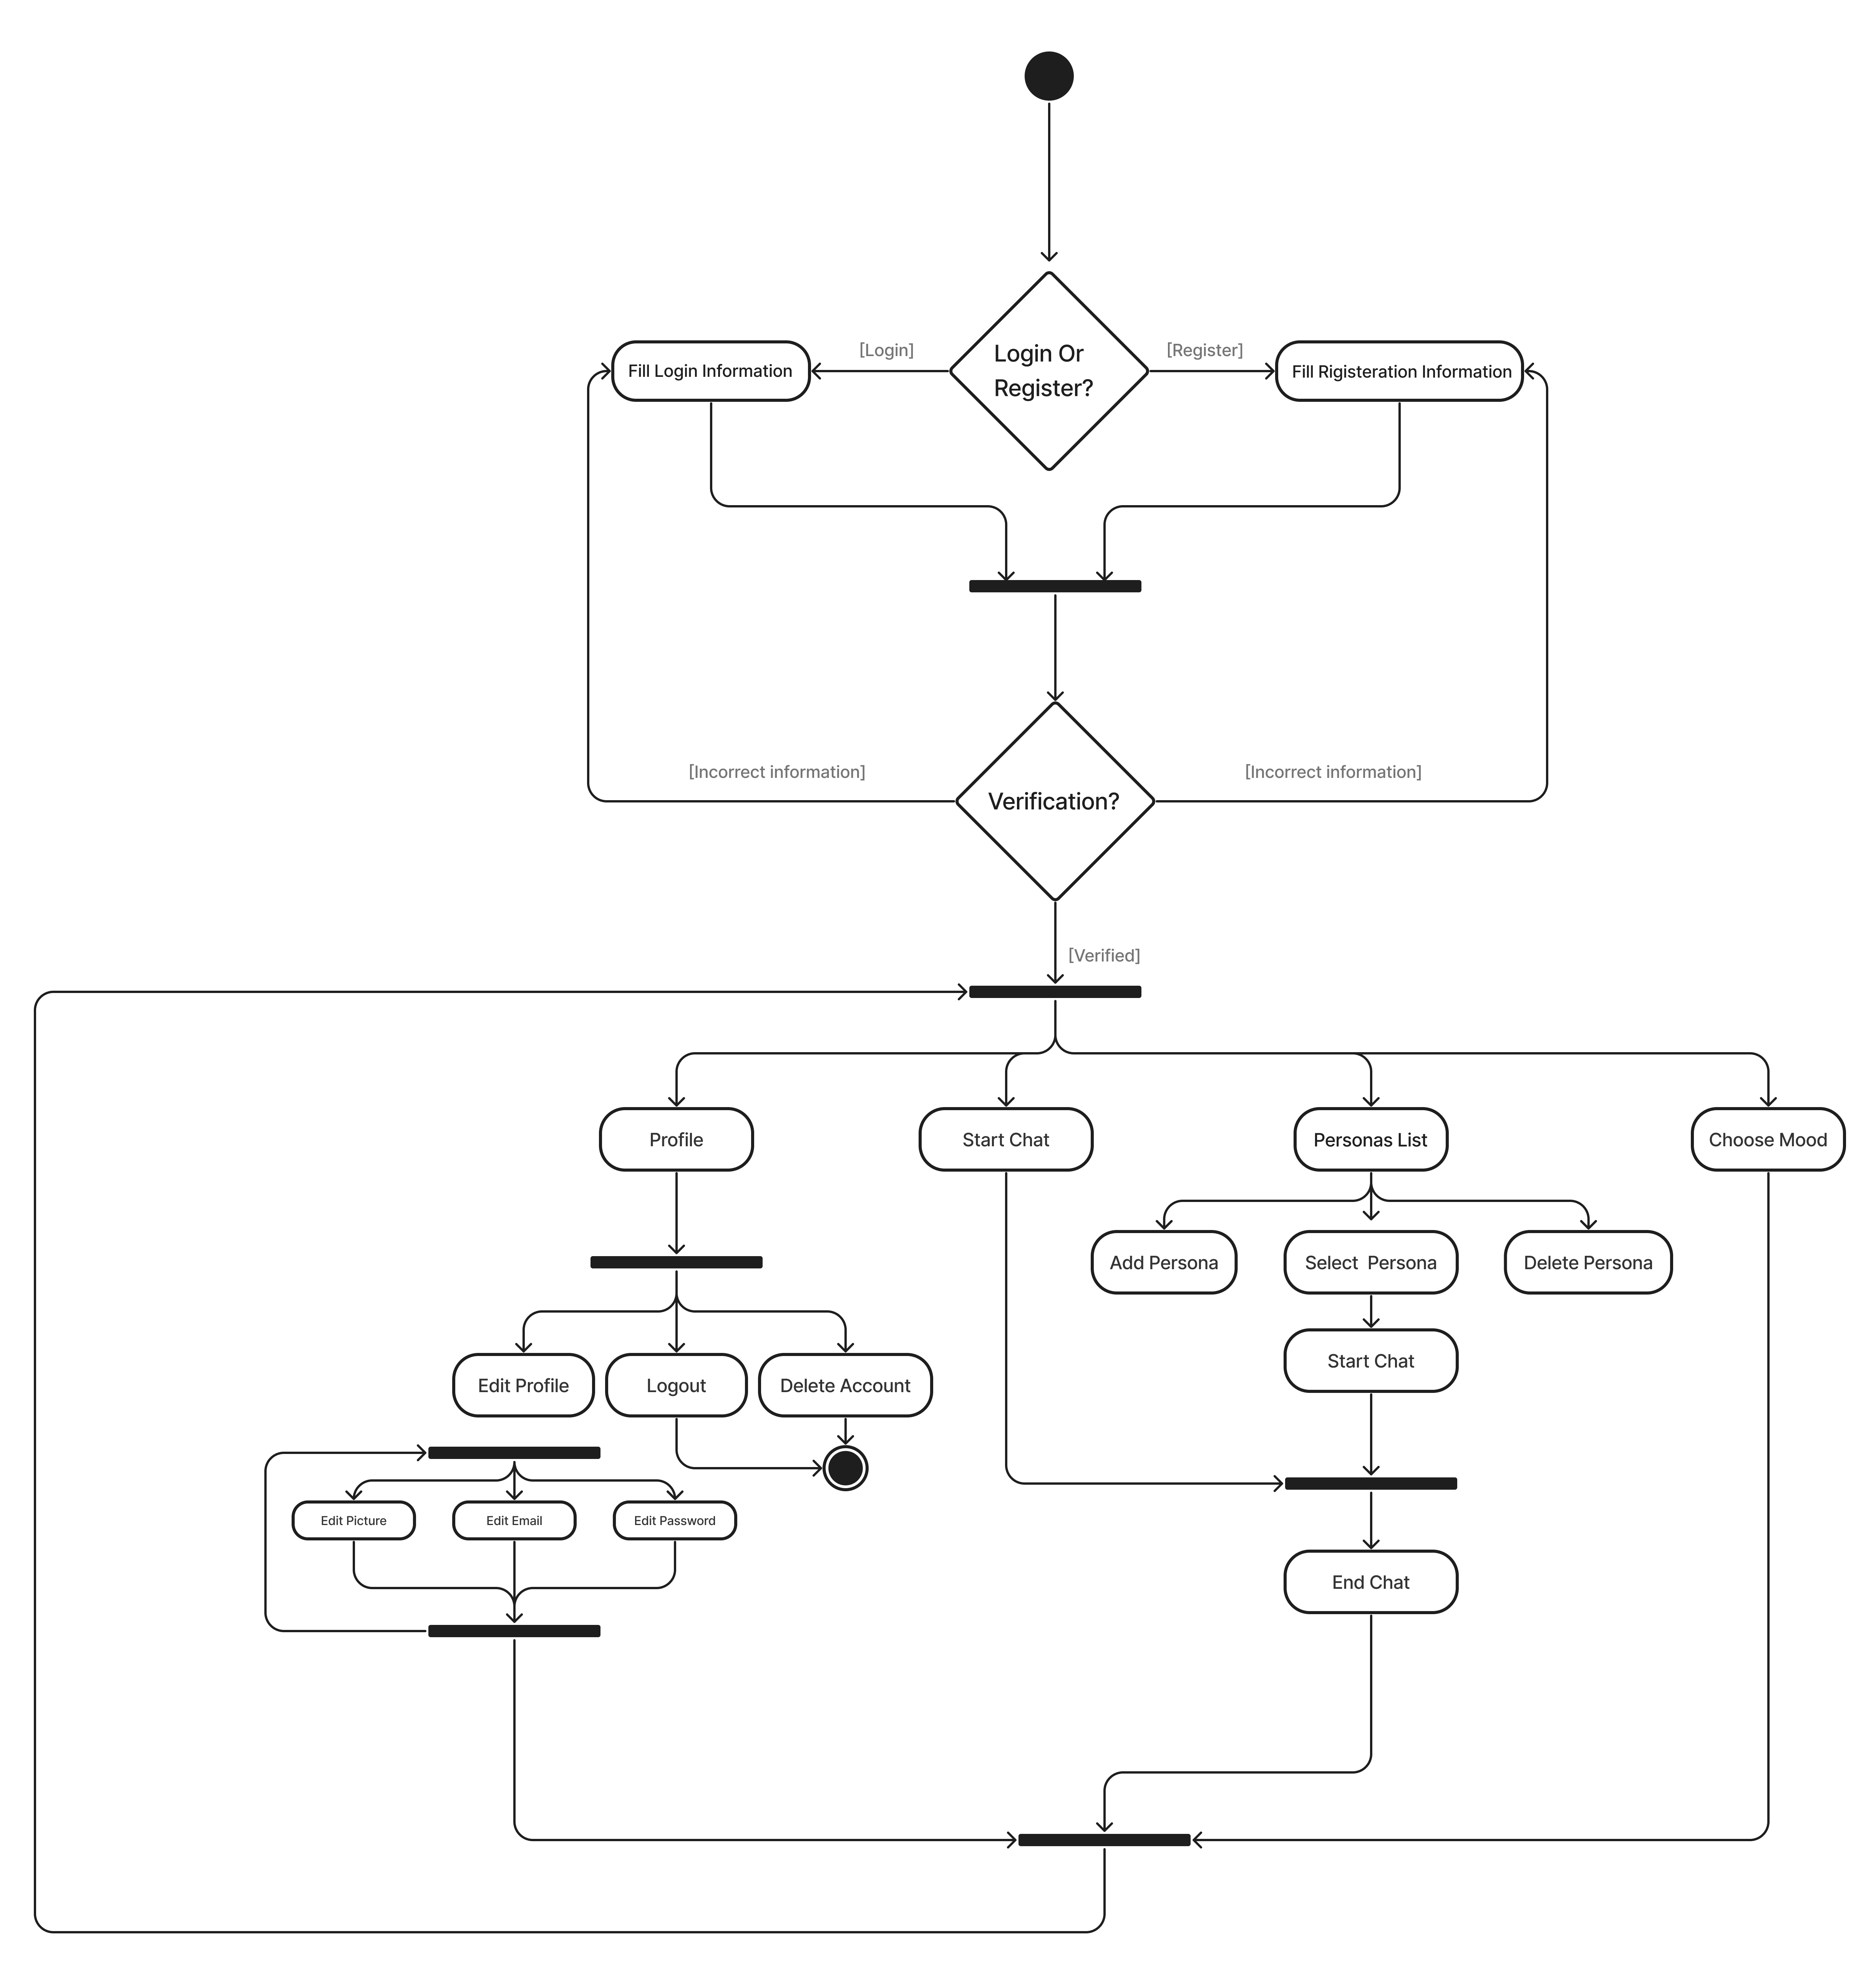
\includegraphics[scale=0.12]{ad}
    \end{center}
\centering
\end{figure}
\newpage
\subsection{User Flow}
\begin{figure}[h]
    \begin{center}
\includegraphics[scale=0.13]{uf}
\end{center}
\centering
\end{figure}

\newpage
\subsection{Block Diagram}
\begin{figure}[h]
    \begin{center}
        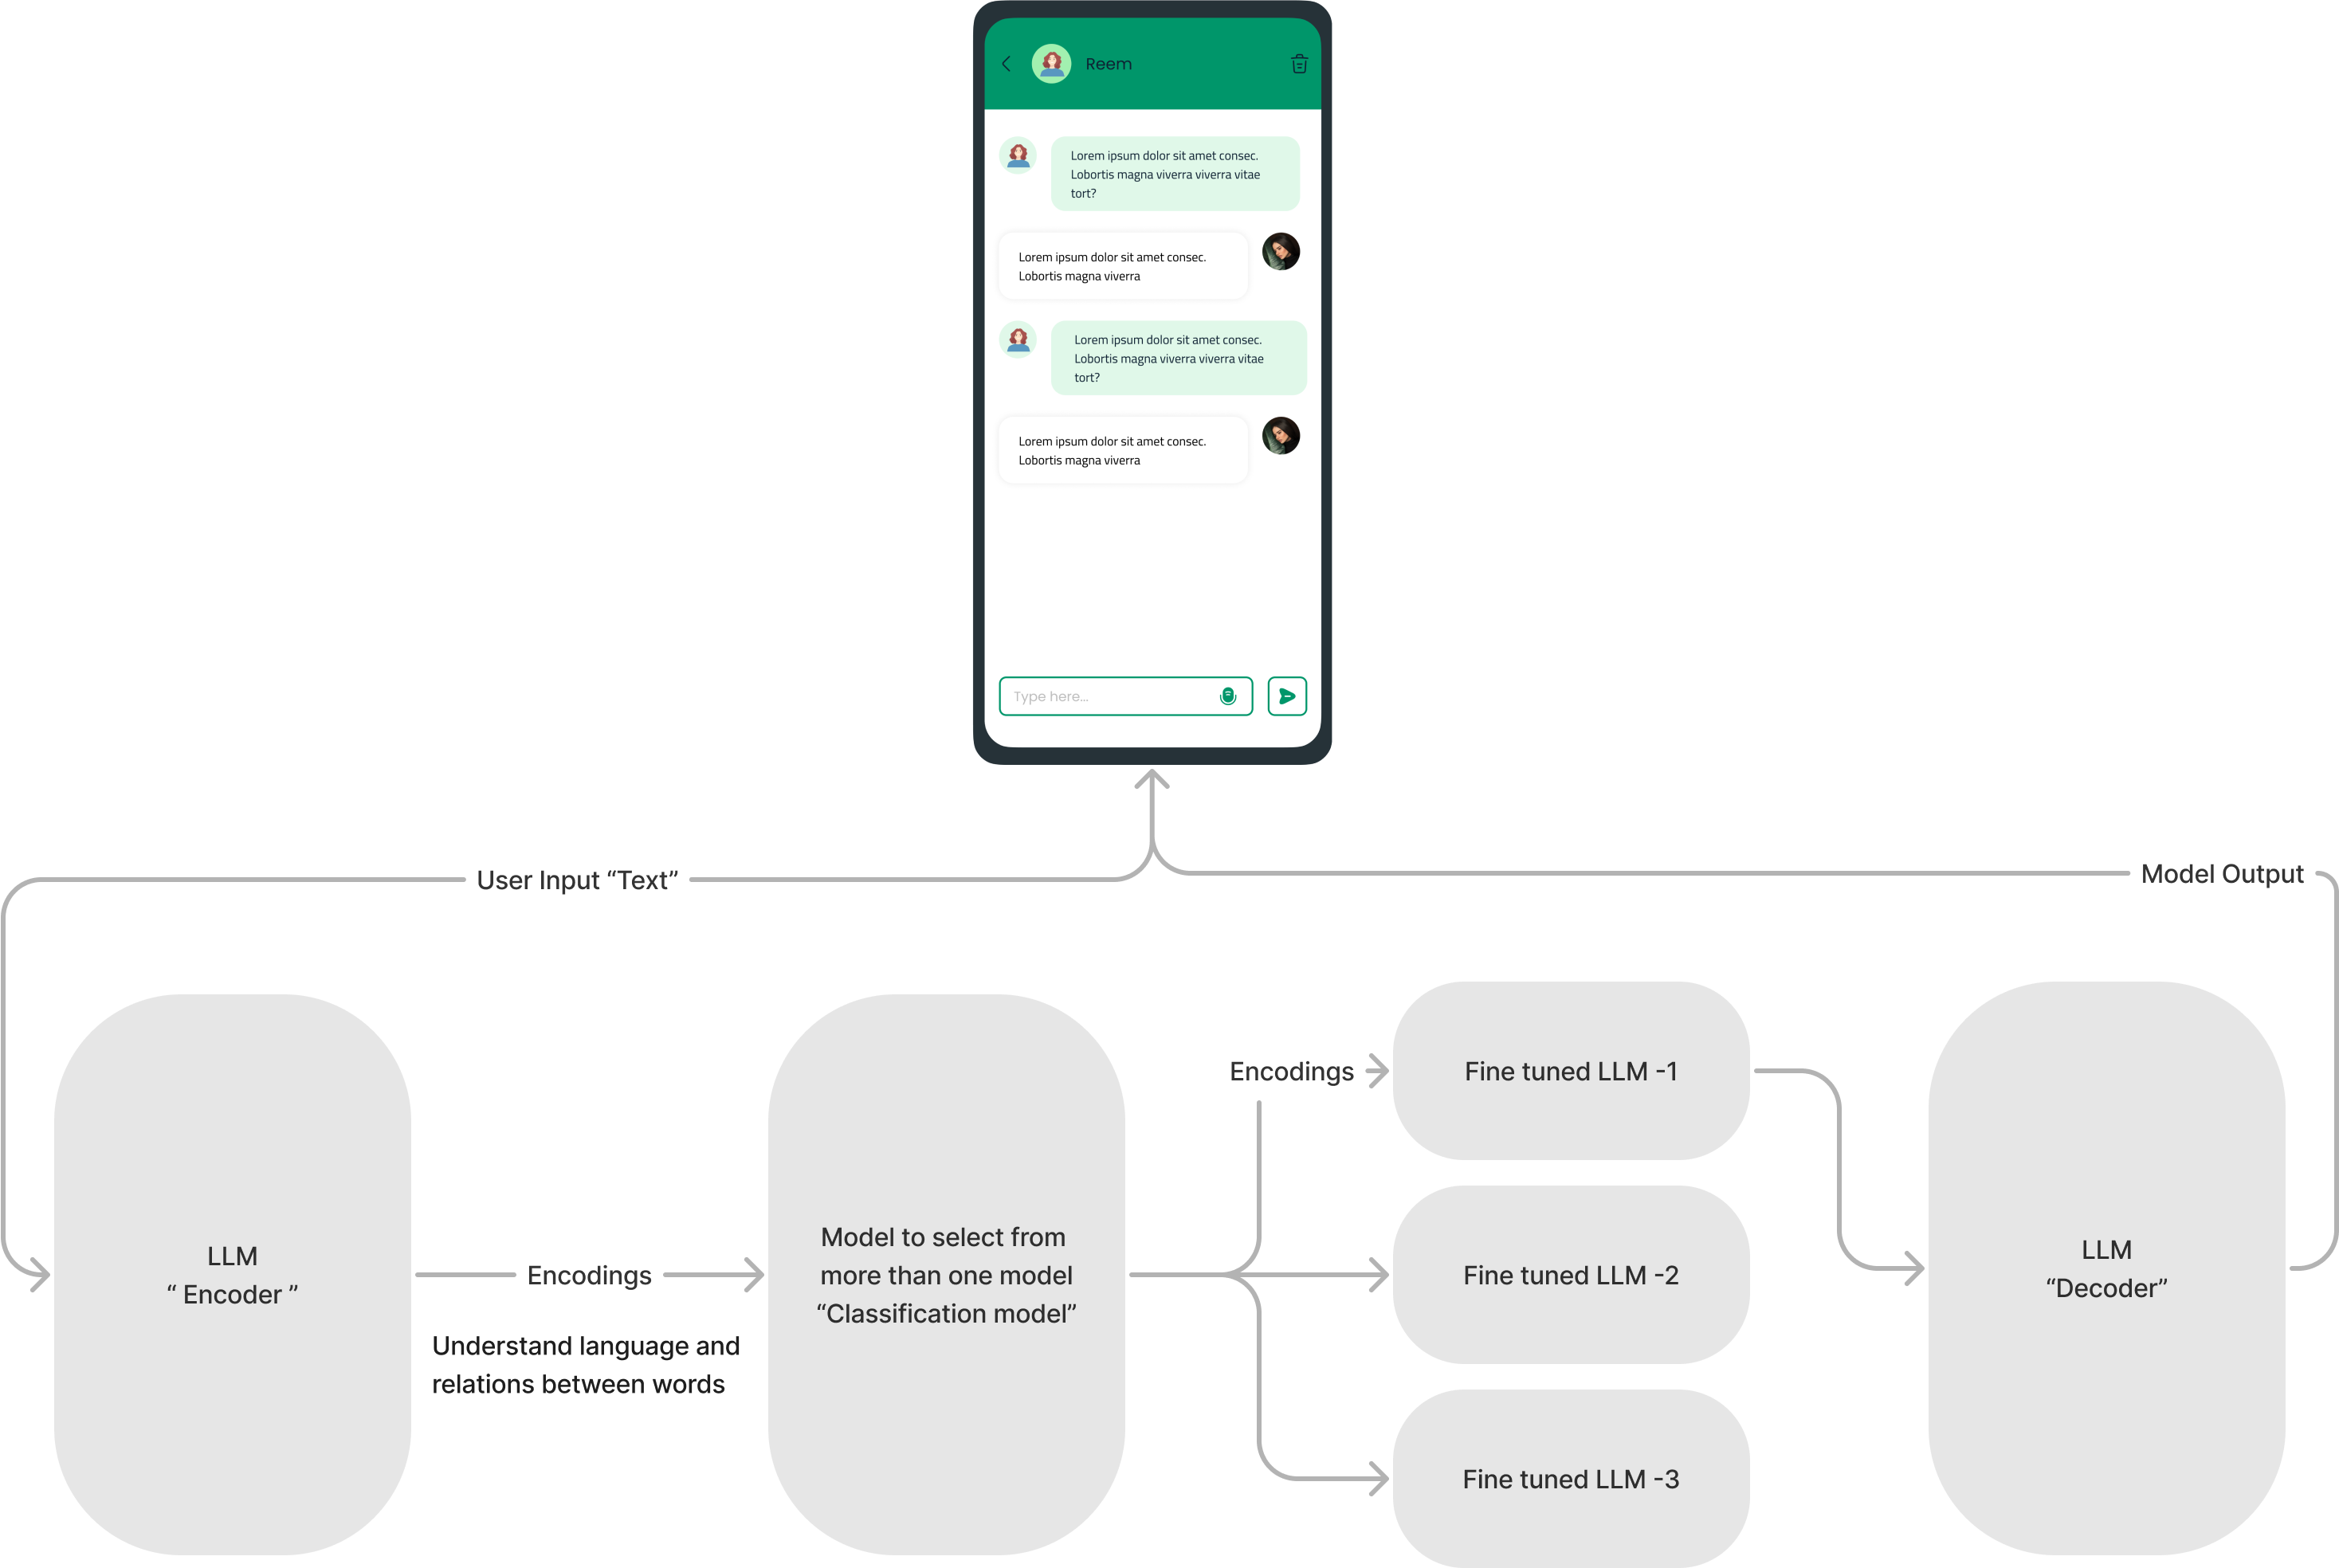
\includegraphics[scale=0.14]{bd}
    \end{center}
\centering
\end{figure}

\newpage
\subsection{Class Diagram}
\begin{figure}[h]
    \begin{center}
        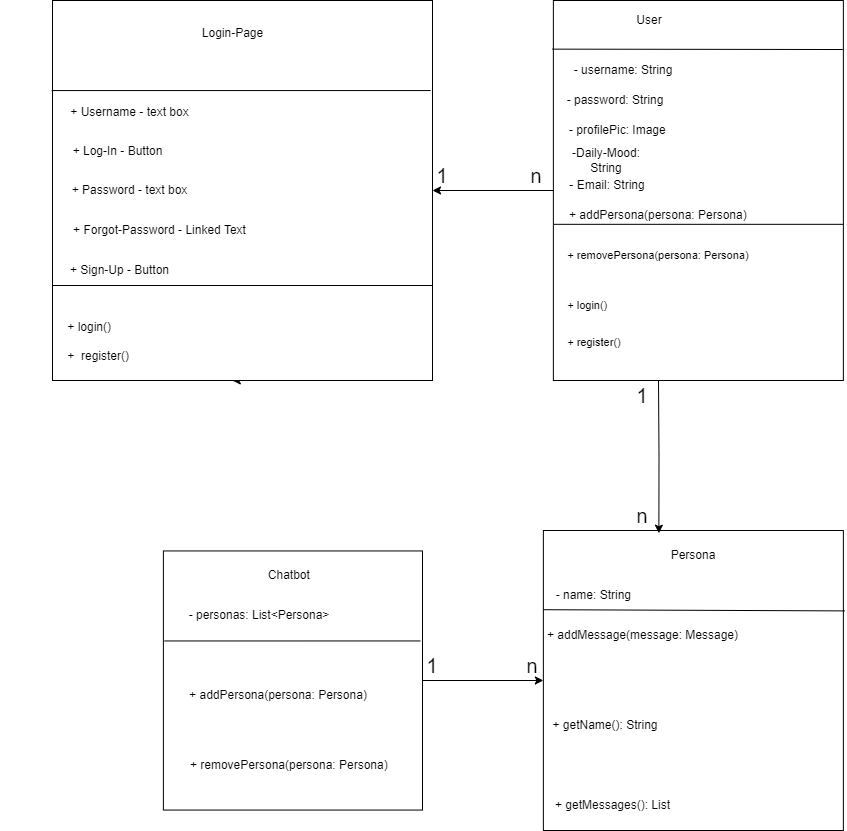
\includegraphics[width=4.5in]{cd}
    \end{center}
\centering
\end{figure}

\newpage
\subsection{Sequence Diagram}
\begin{figure}[h]
    \begin{center}
        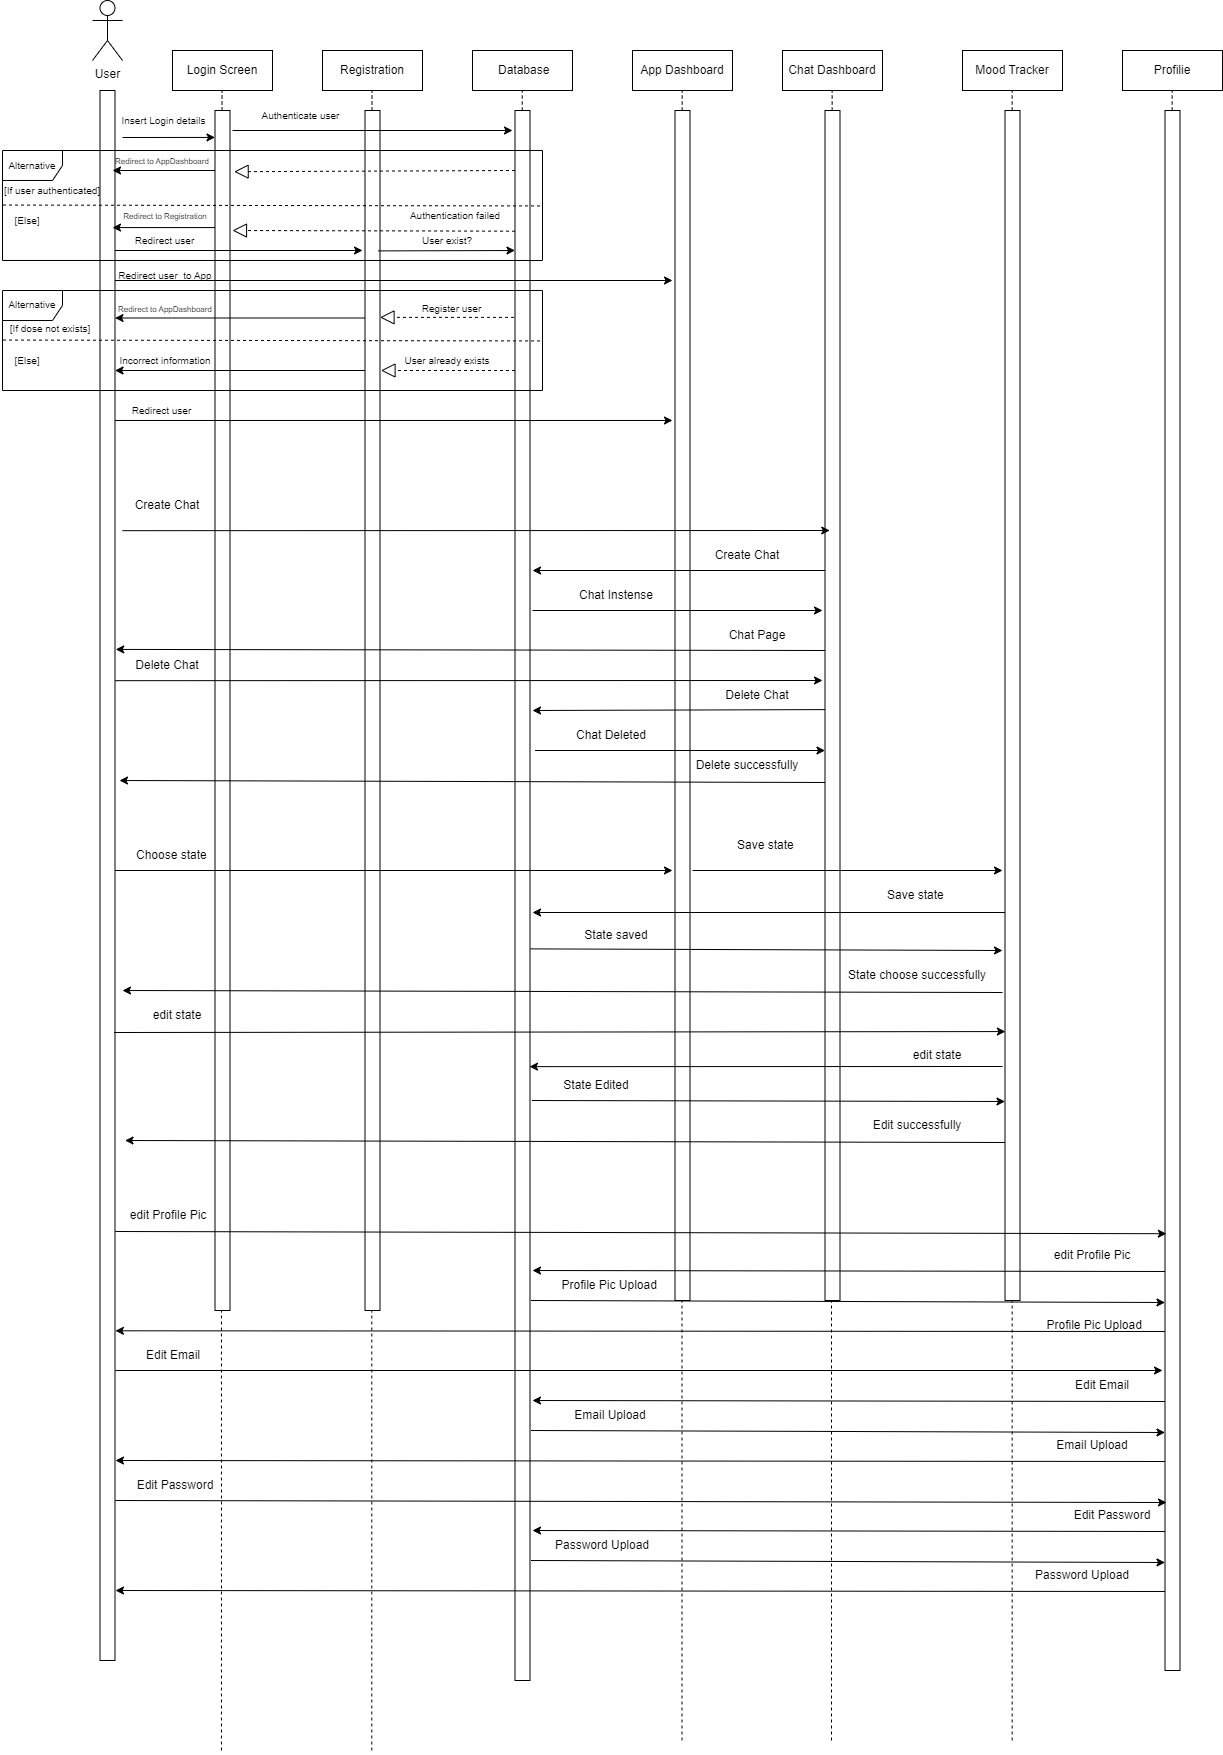
\includegraphics[width=5.0in]{sd}
    \end{center}
\centering
\end{figure}


\newpage
\subsection{Use Case}
\begin{figure}[h]
    \begin{center}
        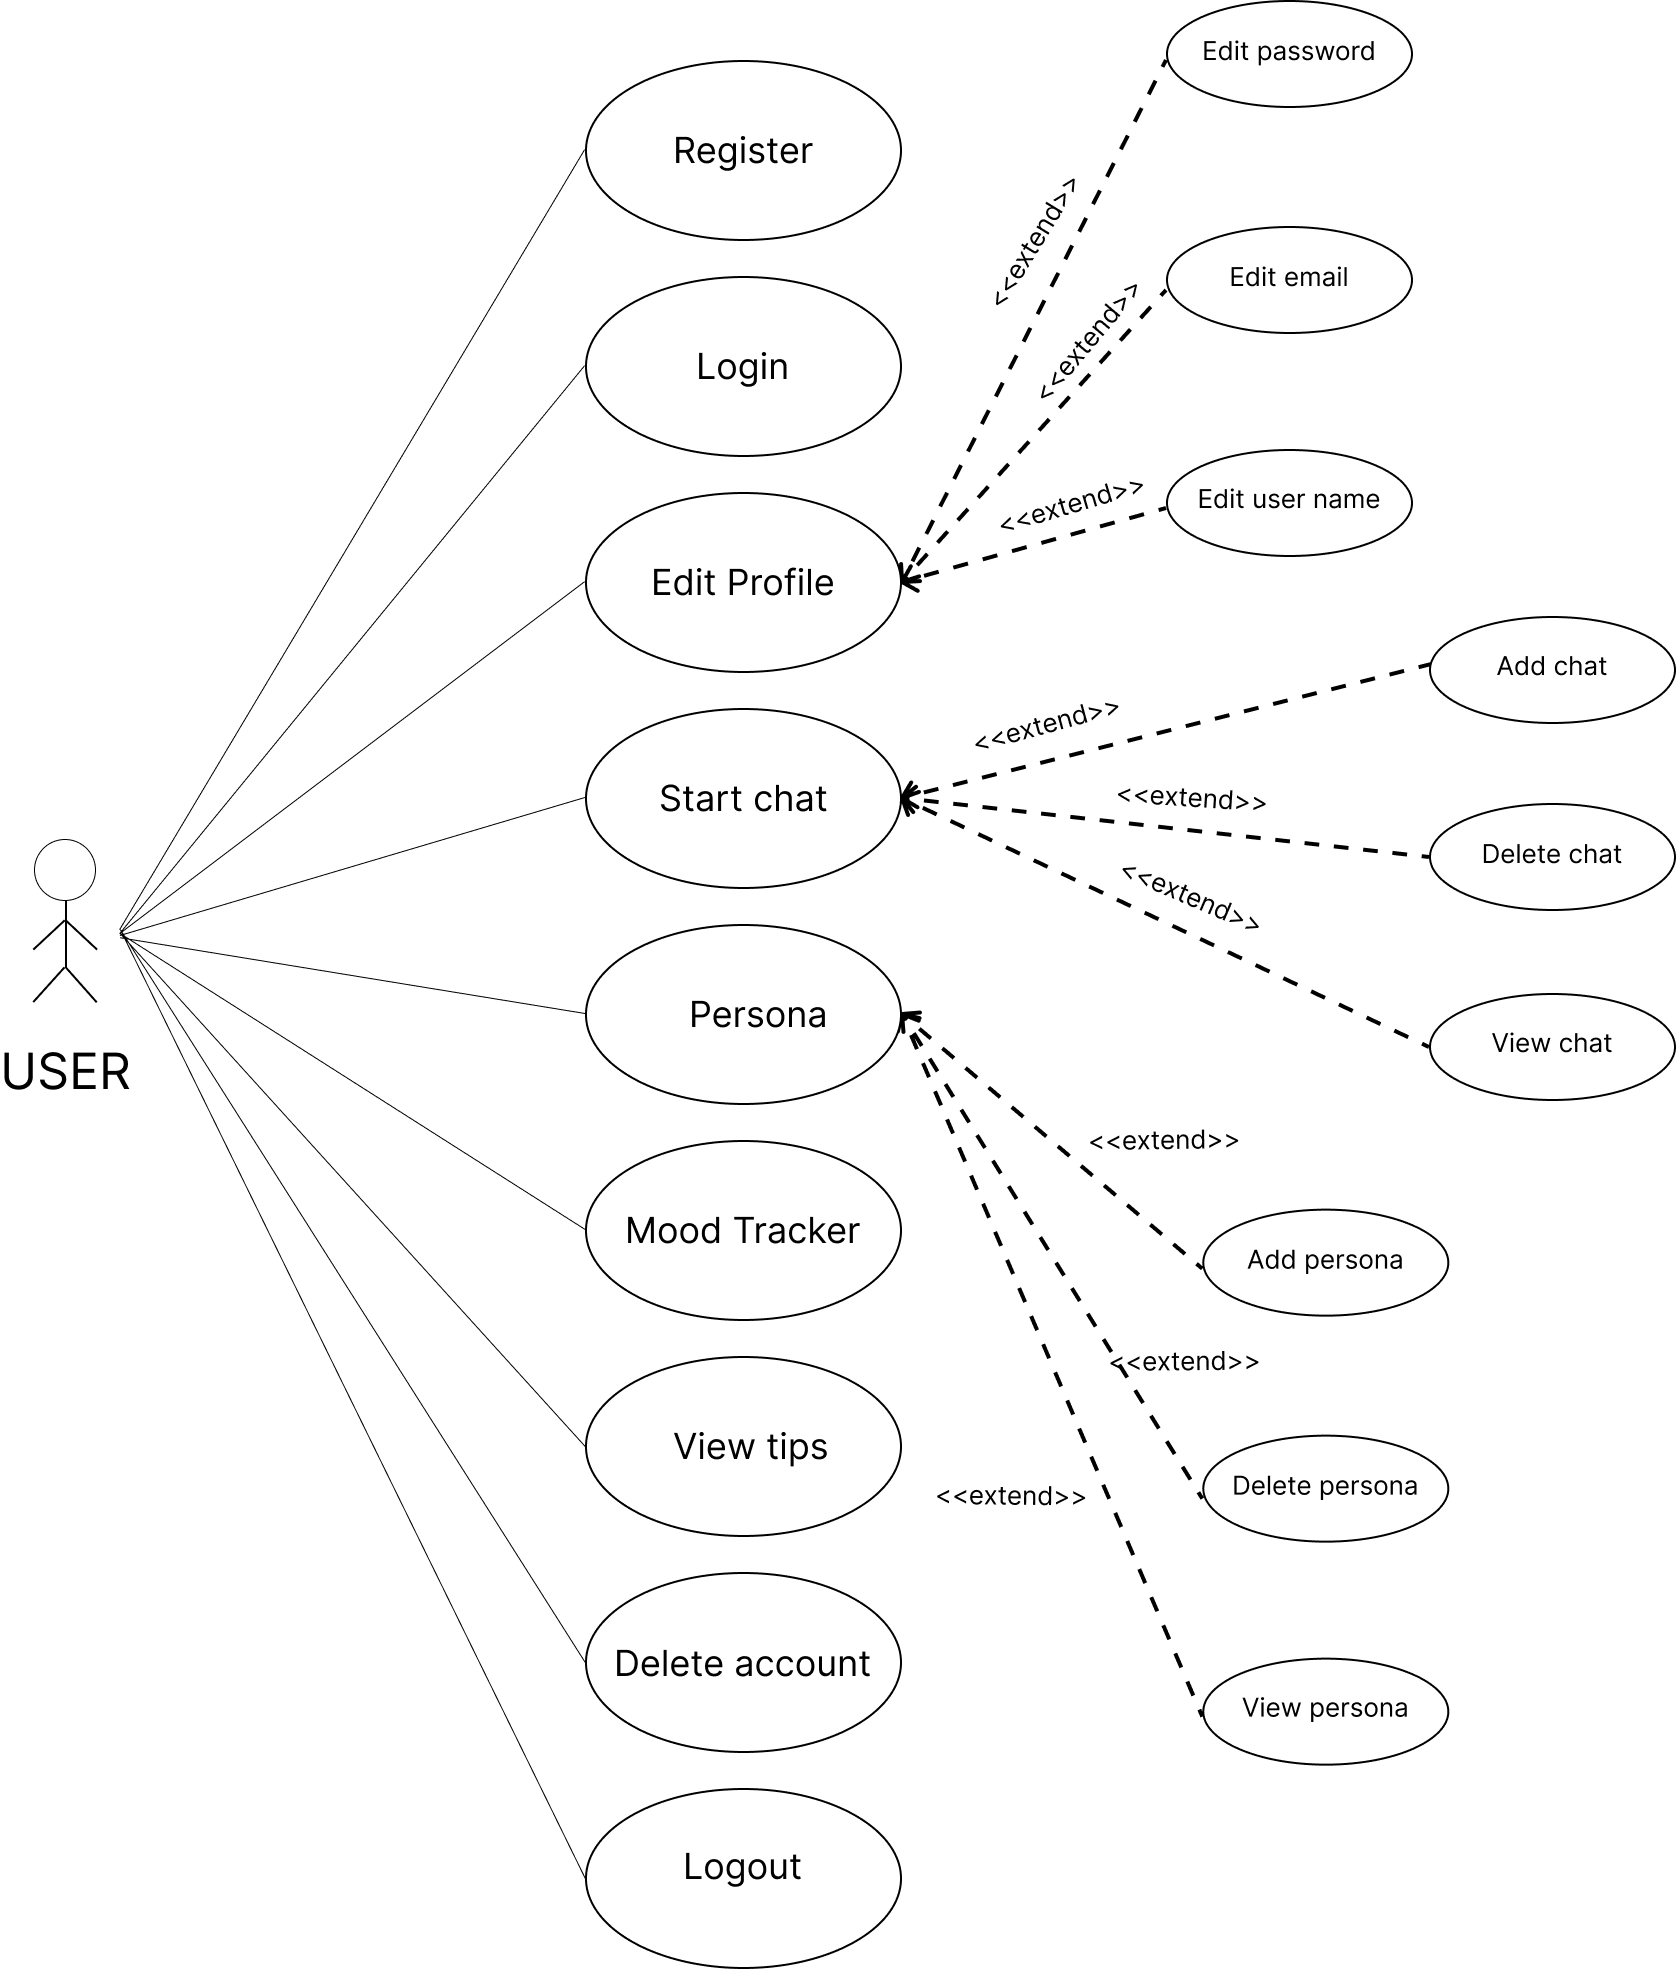
\includegraphics[width=4.5in]{uc}
    \end{center}
\centering
\end{figure}


\newpage
\section{User Interface}
\begin{figure}[h]
    \centering
    \begin{minipage}{0.45\textwidth}
        \centering
{%
\setlength{\fboxsep}{0pt}%
\setlength{\fboxrule}{1pt}%
\fbox{
\includegraphics[width=\textwidth]{a1}}%
}%
    \end{minipage}
    \hfill
    \begin{minipage}{0.45\textwidth}
        \centering
{%
\setlength{\fboxsep}{0pt}%
\setlength{\fboxrule}{1pt}%
\fbox{
\includegraphics[width=\textwidth]{a2}}%
}%
    \end{minipage}
\end{figure}




\begin{figure}[htbp]
    \centering

    \begin{minipage}[b]{0.45\textwidth}
        \centering
{%
\setlength{\fboxsep}{0pt}%
\setlength{\fboxrule}{1pt}%
\fbox{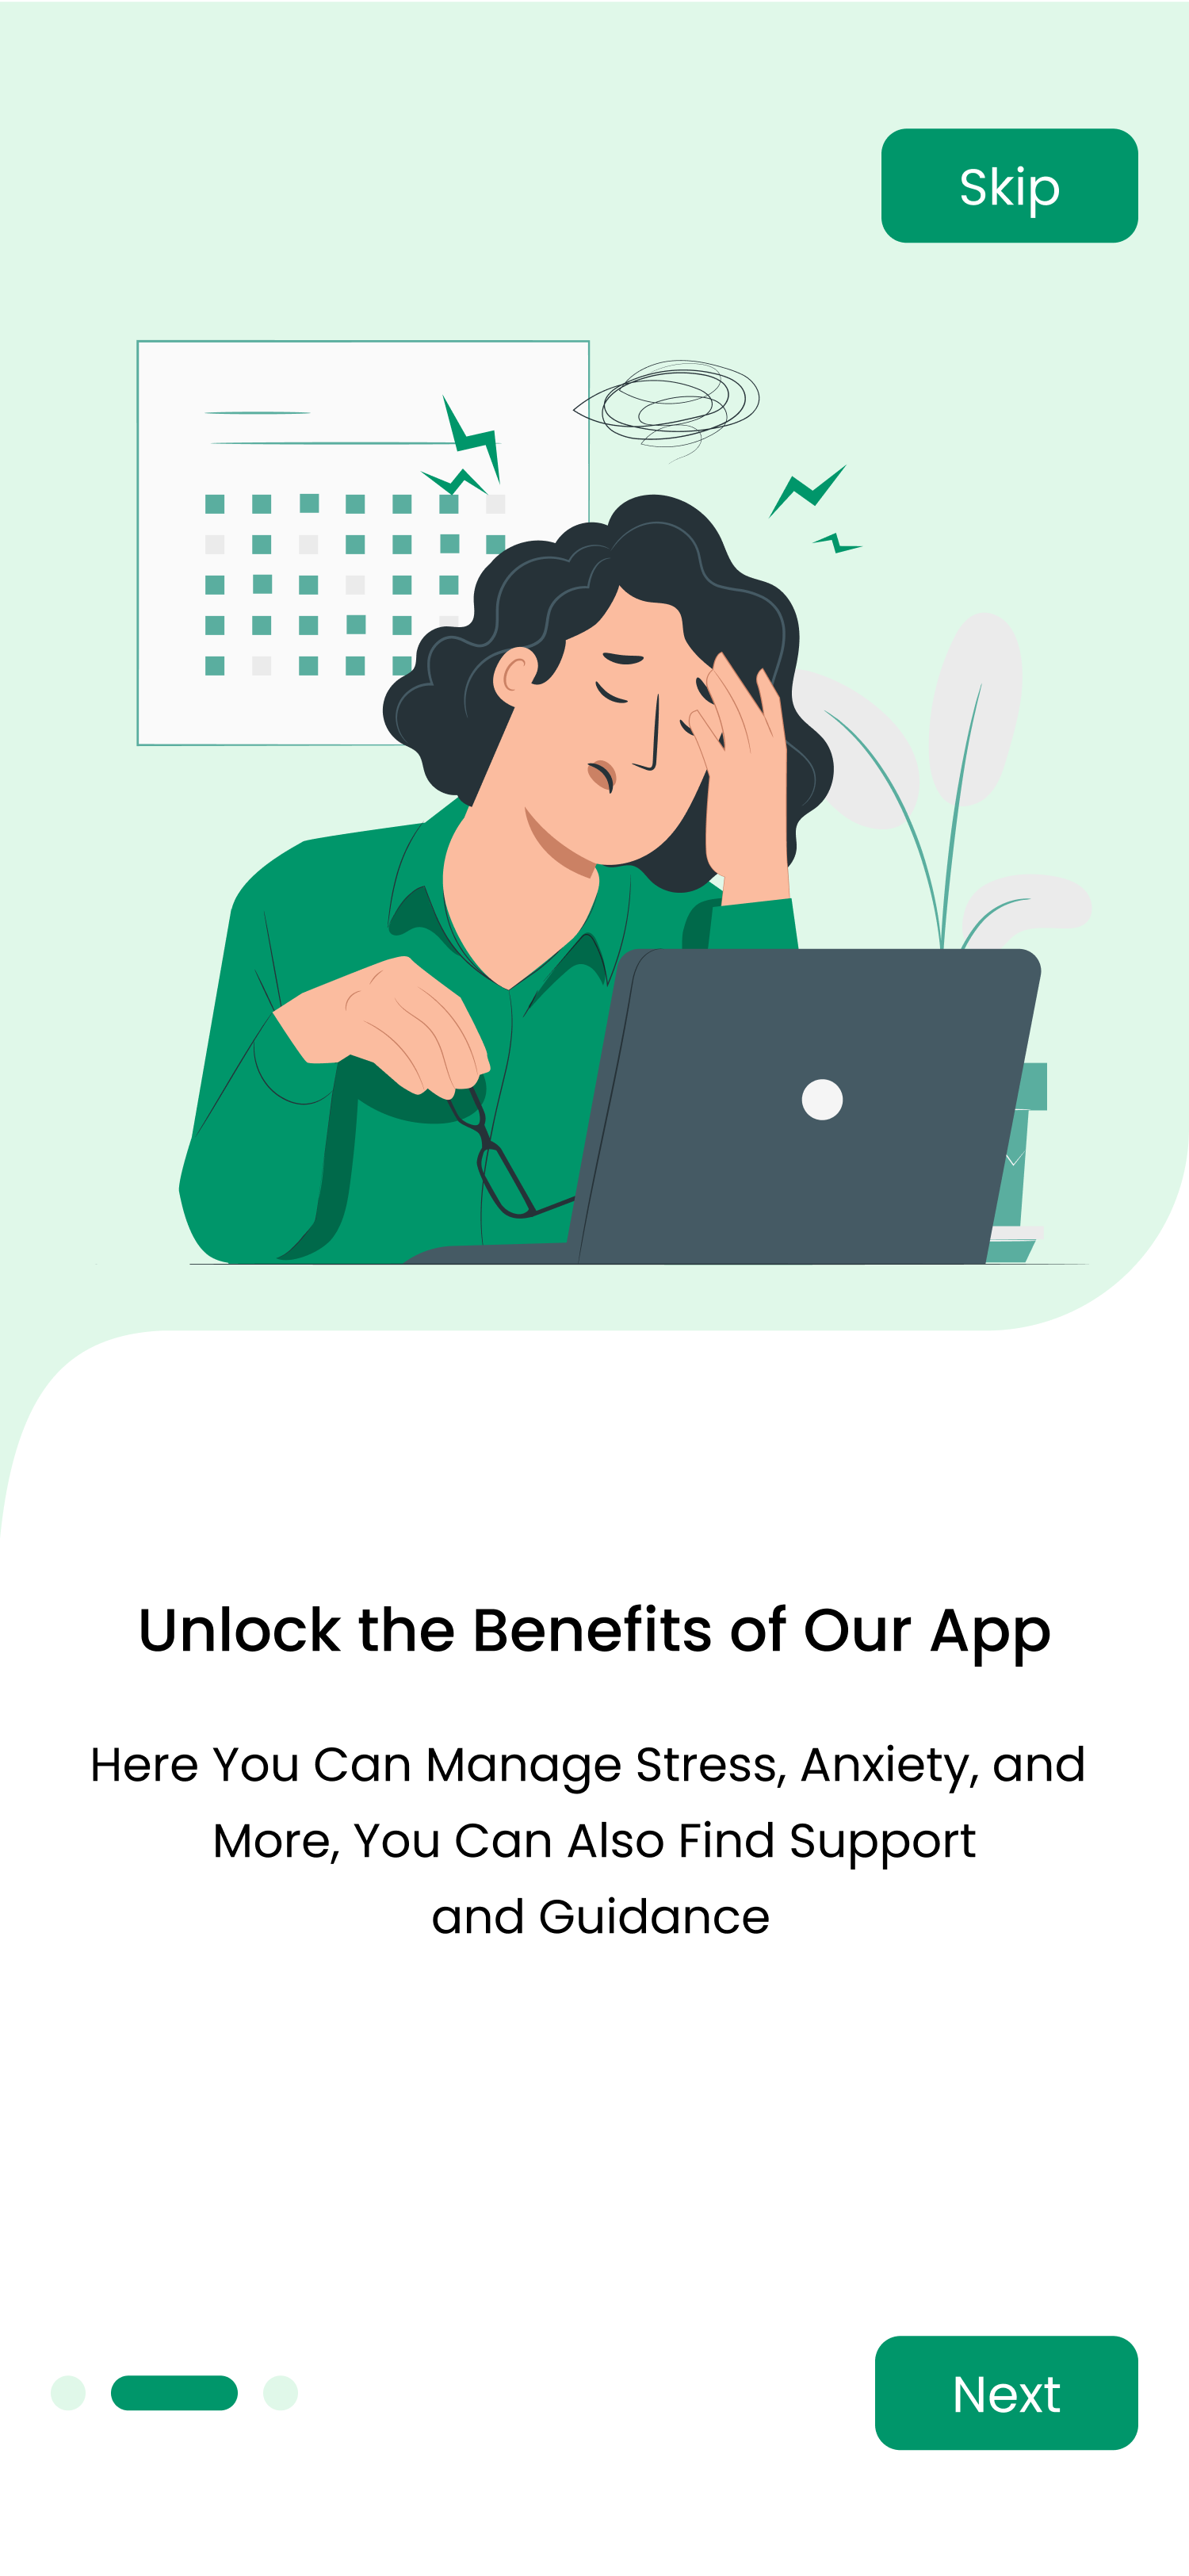
\includegraphics[width=\textwidth]{a4}}%
}%
    \end{minipage}
    \hfill
    \begin{minipage}[b]{0.45\textwidth}
        \centering
{%
\setlength{\fboxsep}{0pt}%
\setlength{\fboxrule}{1pt}%
\fbox{
\includegraphics[width=\textwidth]{a5}}%
}%
    \end{minipage}
\end{figure}





\begin{figure}[htbp]
    \centering

    \begin{minipage}[b]{0.45\textwidth}
        \centering
{%
\setlength{\fboxsep}{0pt}%
\setlength{\fboxrule}{1pt}%
\fbox{
\includegraphics[width=\textwidth]{a6}}%
}%
    \end{minipage}
    \hfill
    \begin{minipage}[b]{0.45\textwidth}
        \centering
{%
\setlength{\fboxsep}{0pt}%
\setlength{\fboxrule}{1pt}%
\fbox{
\includegraphics[width=\textwidth]{a8}}%
}%
    \end{minipage}
\end{figure}





\begin{figure}[htbp]
    \centering

    \begin{minipage}[b]{0.45\textwidth}
        \centering
{%
\setlength{\fboxsep}{0pt}%
\setlength{\fboxrule}{1pt}%
\fbox{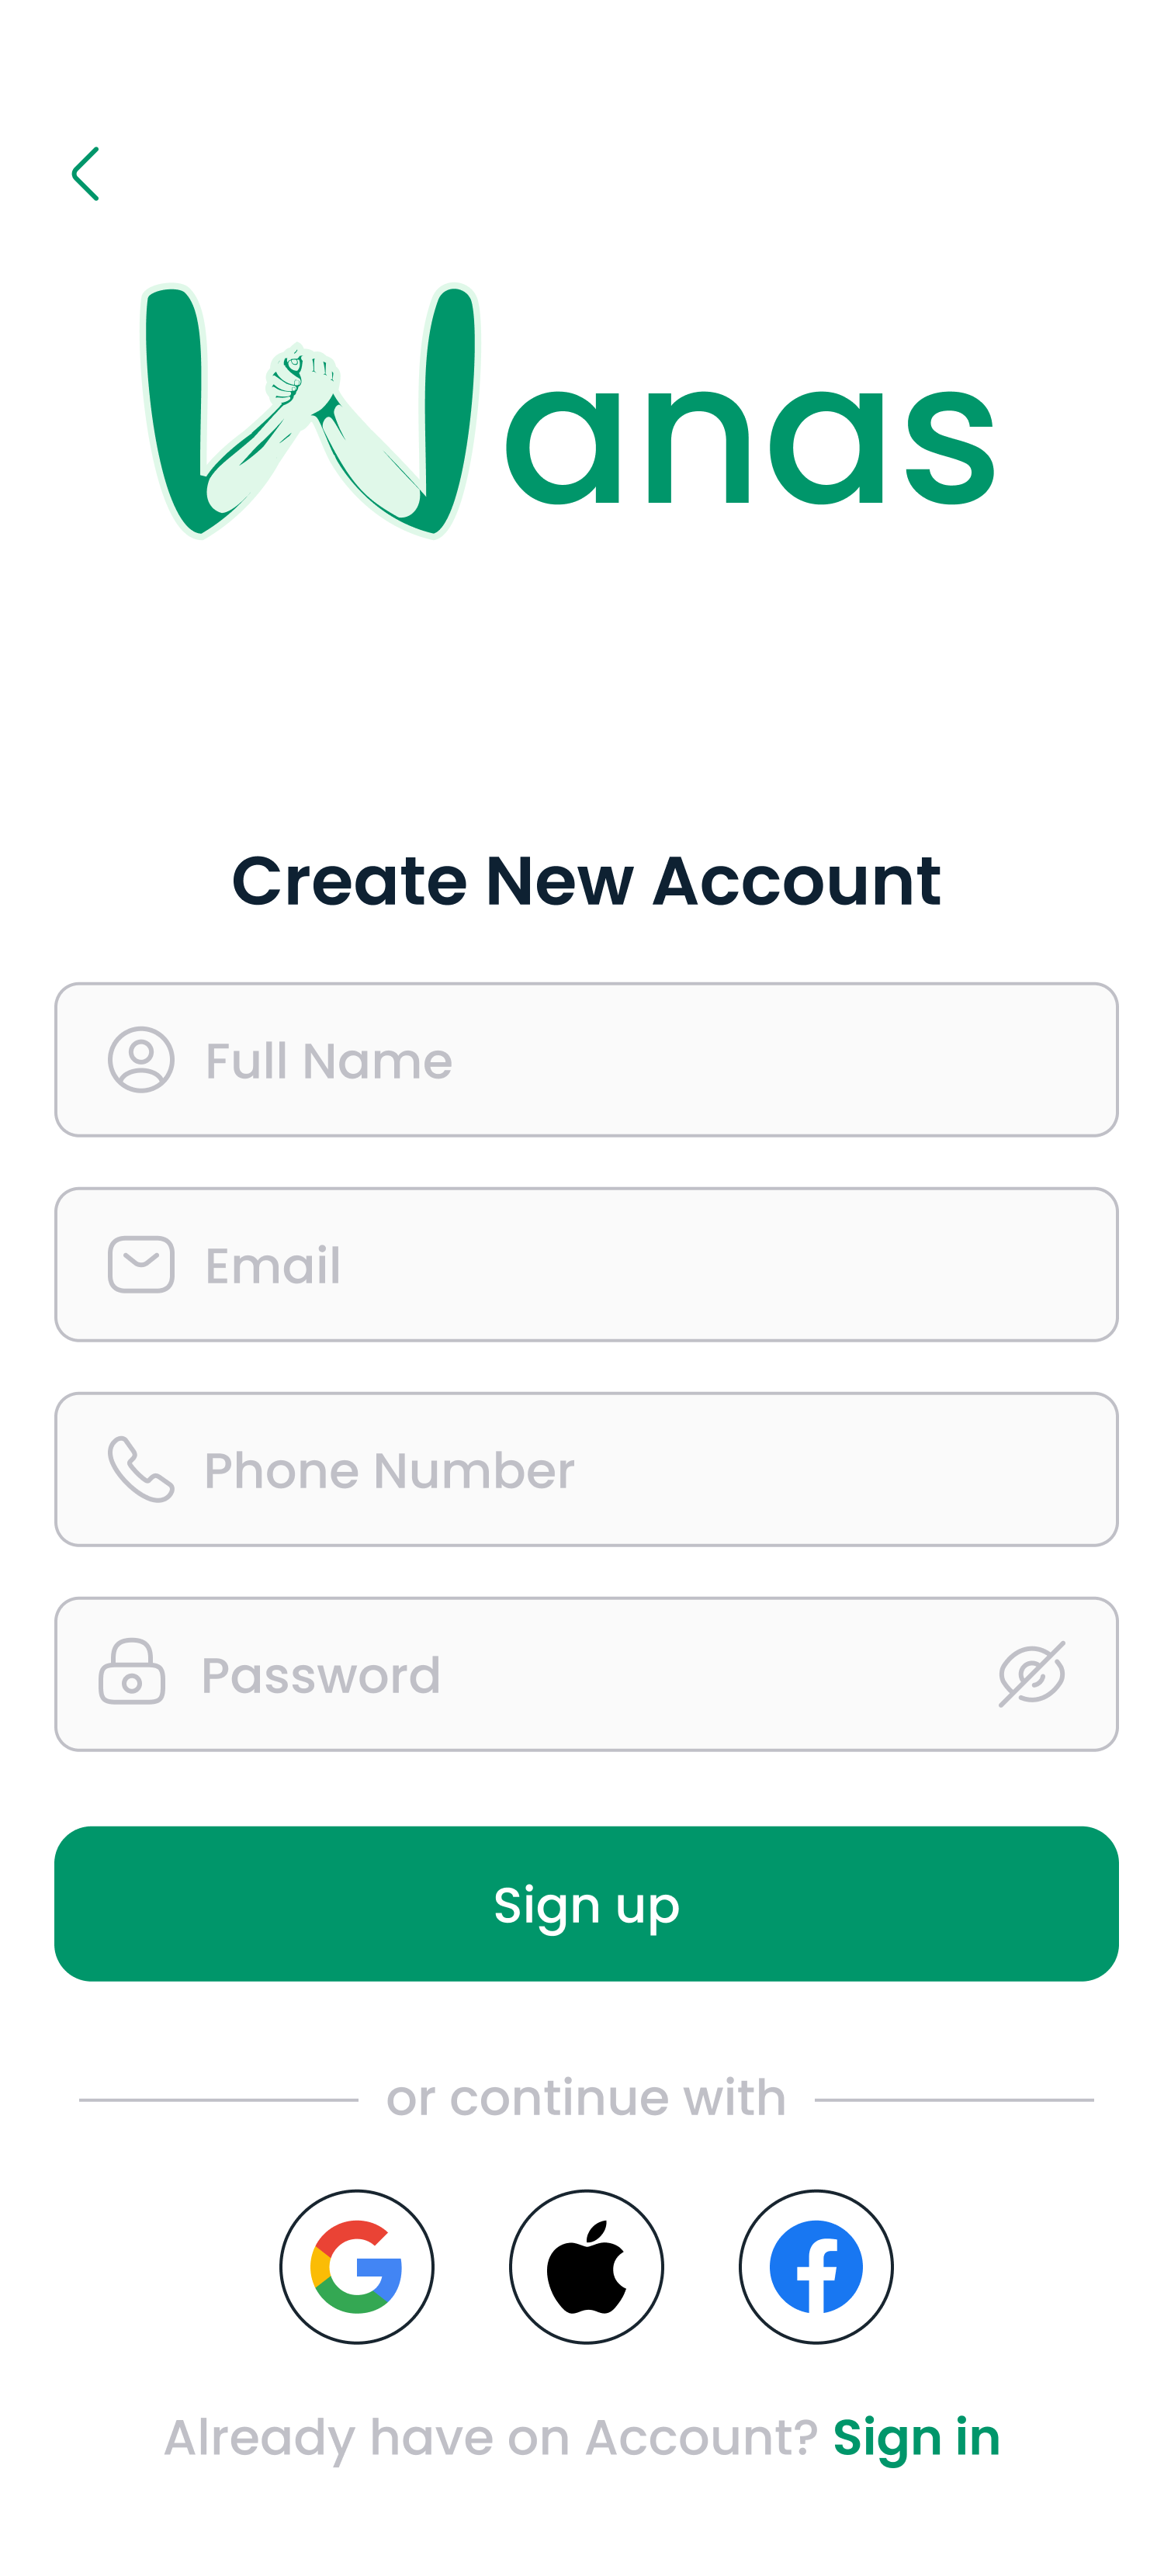
\includegraphics[width=\textwidth]{a9}}%
}%
    \end{minipage}
    \hfill
    \begin{minipage}[b]{0.45\textwidth}
        \centering
{%
\setlength{\fboxsep}{0pt}%
\setlength{\fboxrule}{1pt}%
\fbox{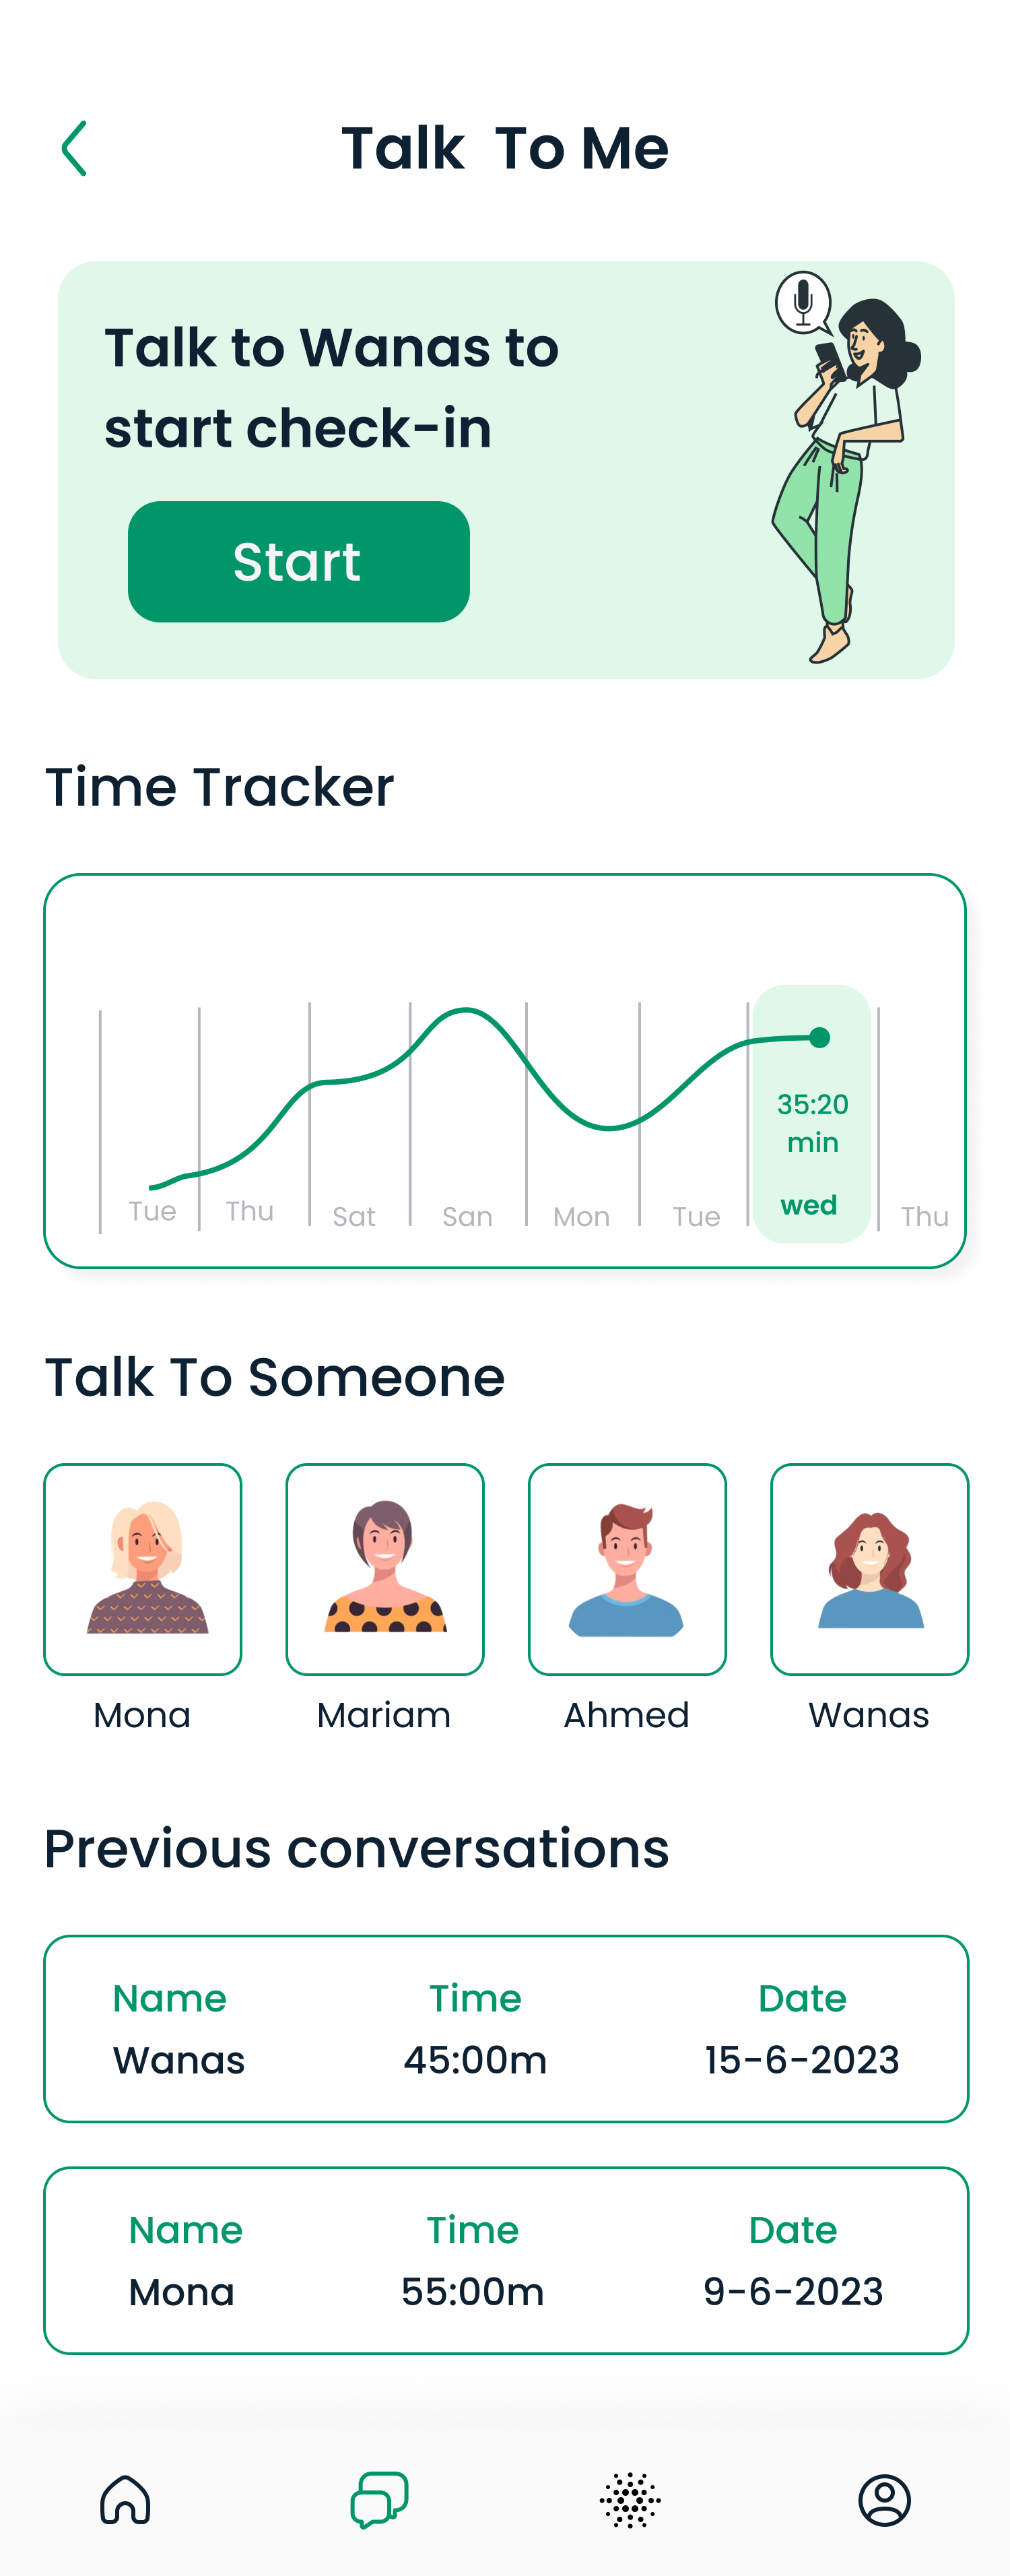
\includegraphics[width=\textwidth]{a10}}%
}%
    \end{minipage}
\end{figure}






\begin{figure}[htbp]
    \centering

    \begin{minipage}[b]{0.45\textwidth}
        \centering
{%
\setlength{\fboxsep}{0pt}%
\setlength{\fboxrule}{1pt}%
\fbox{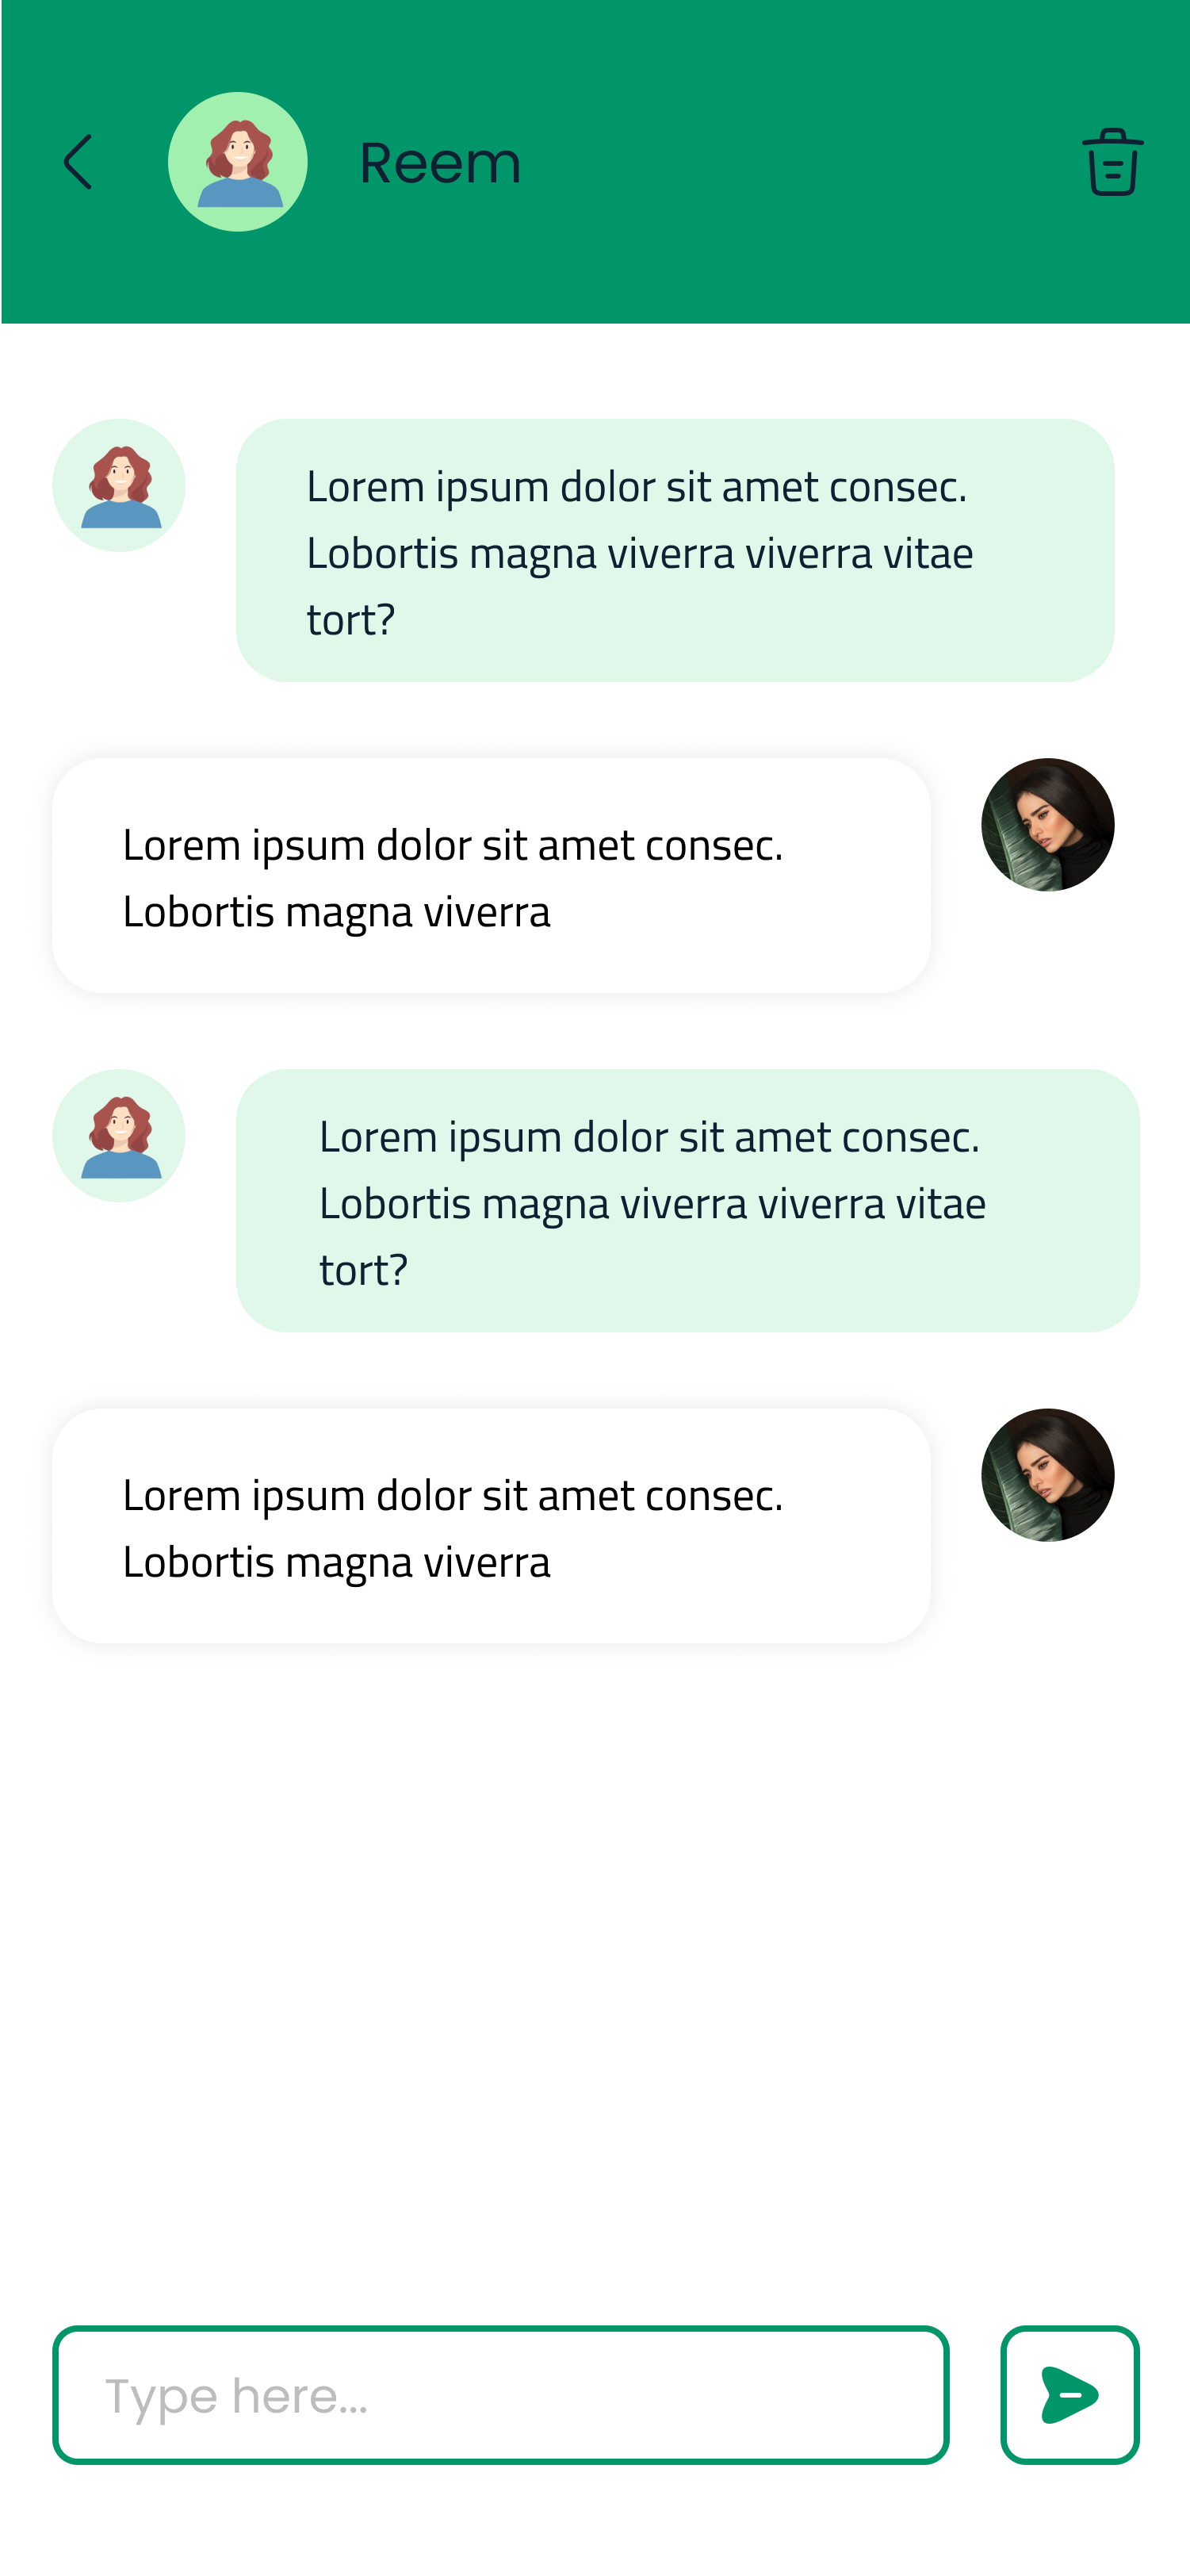
\includegraphics[width=\textwidth]{a11}}%
}%
    \end{minipage}
    \hfill
    \begin{minipage}[b]{0.45\textwidth}
        \centering
{%
\setlength{\fboxsep}{0pt}%
\setlength{\fboxrule}{1pt}%
\fbox{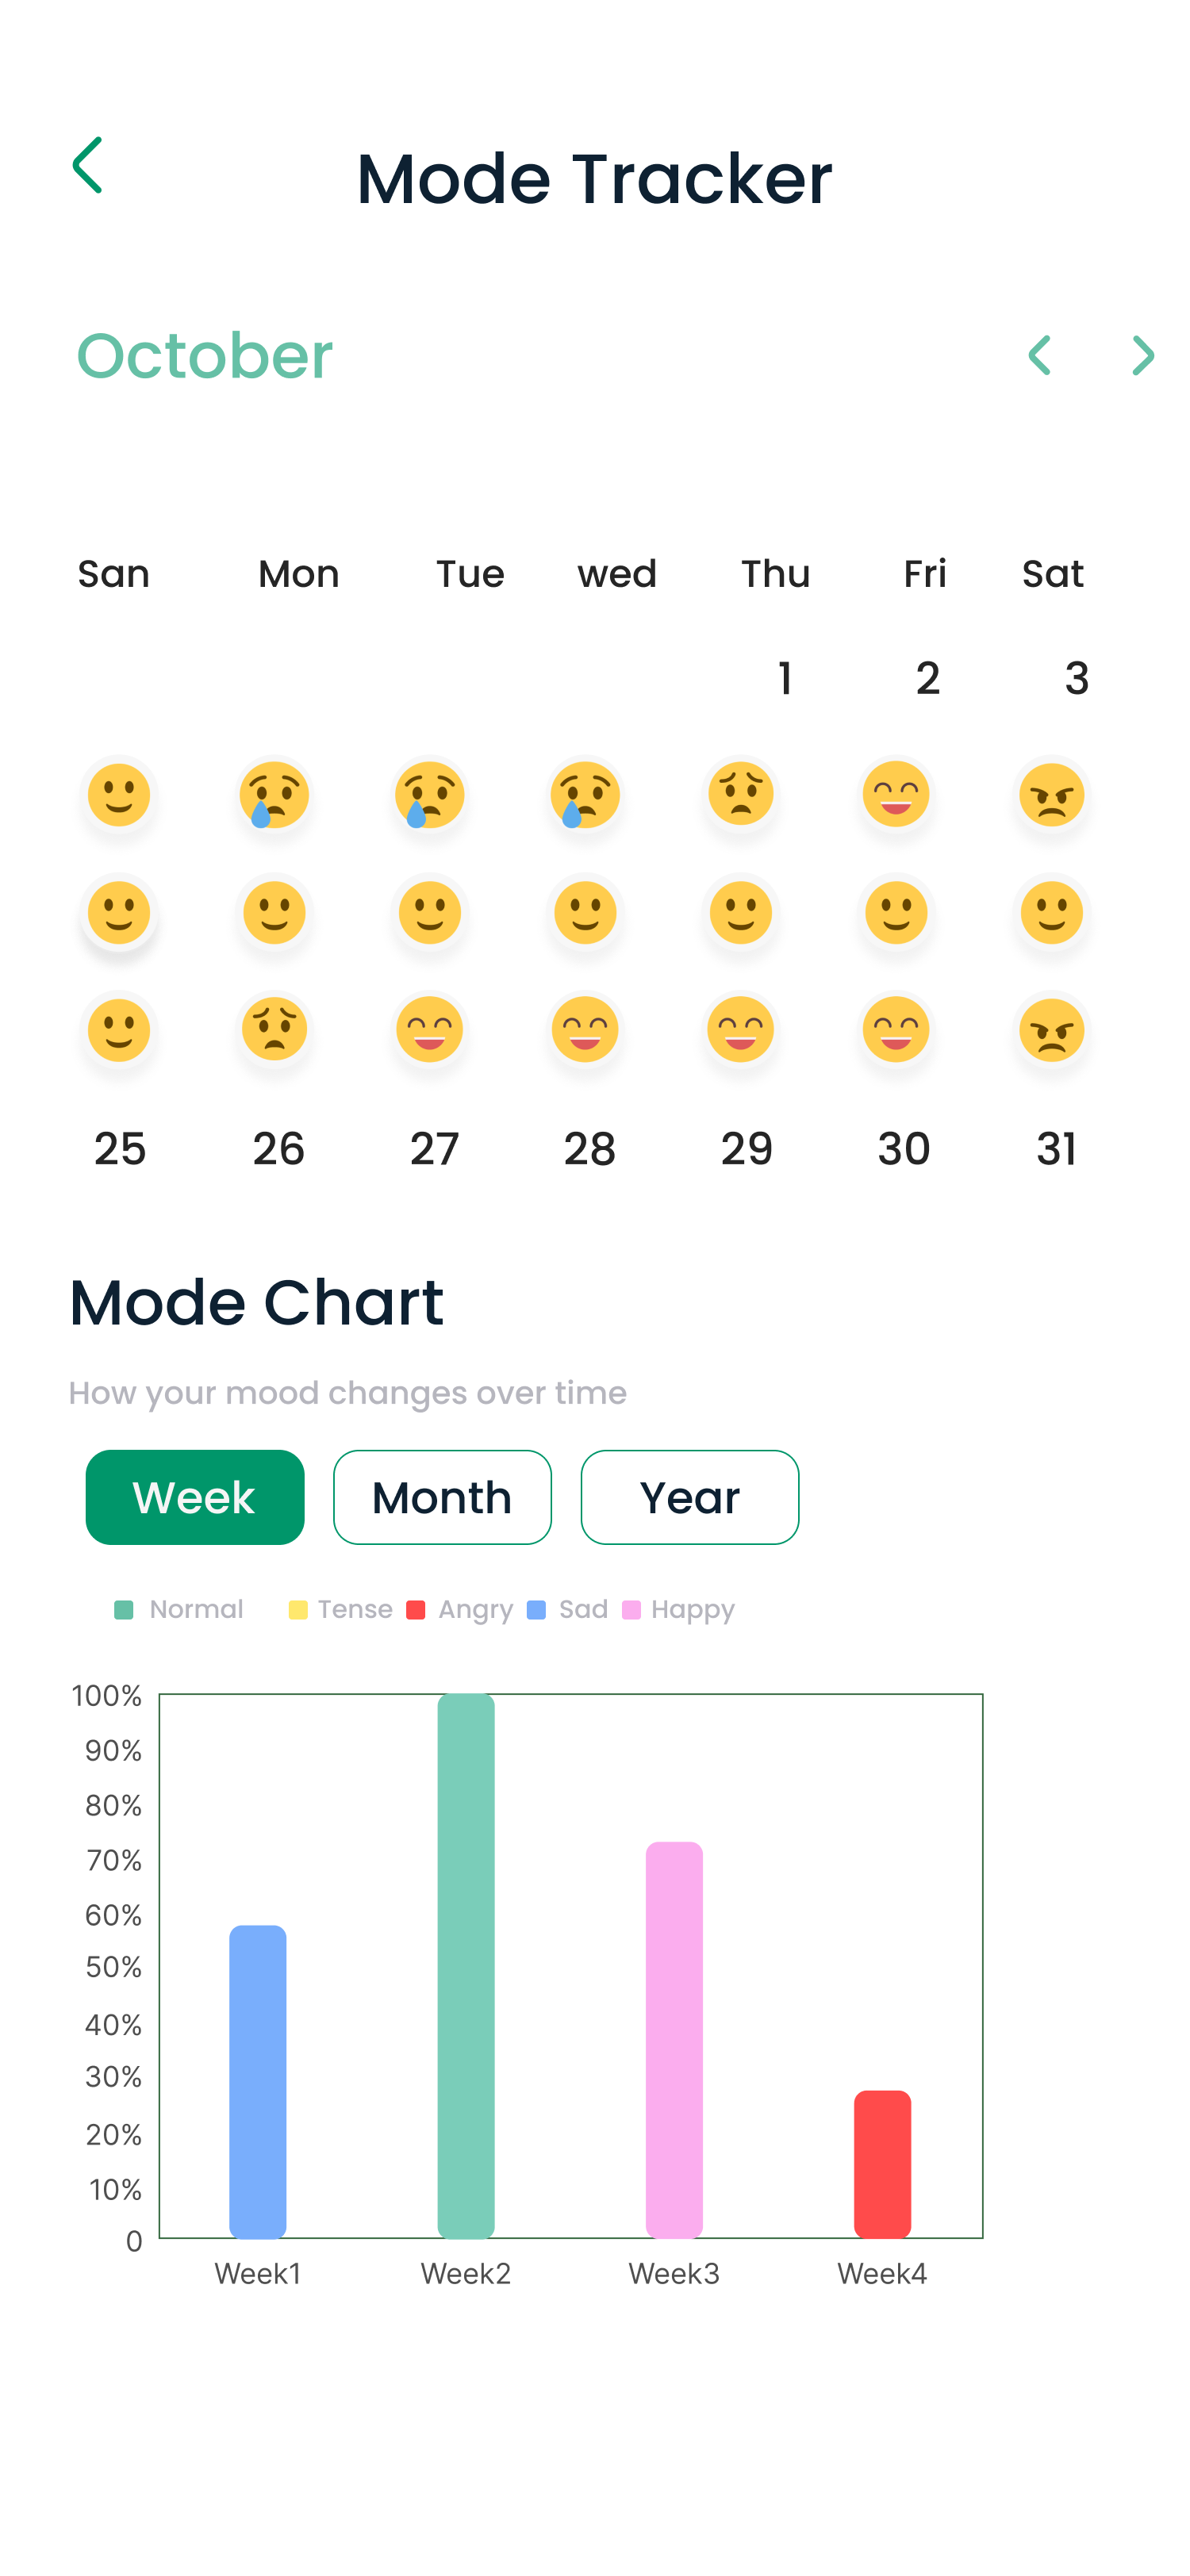
\includegraphics[width=\textwidth]{a12}}%
}%
    \end{minipage}
\end{figure}






\begin{figure}[htbp]
    \centering

    \begin{minipage}[b]{0.45\textwidth}
        \centering
{%
\setlength{\fboxsep}{0pt}%
\setlength{\fboxrule}{1pt}%
\fbox{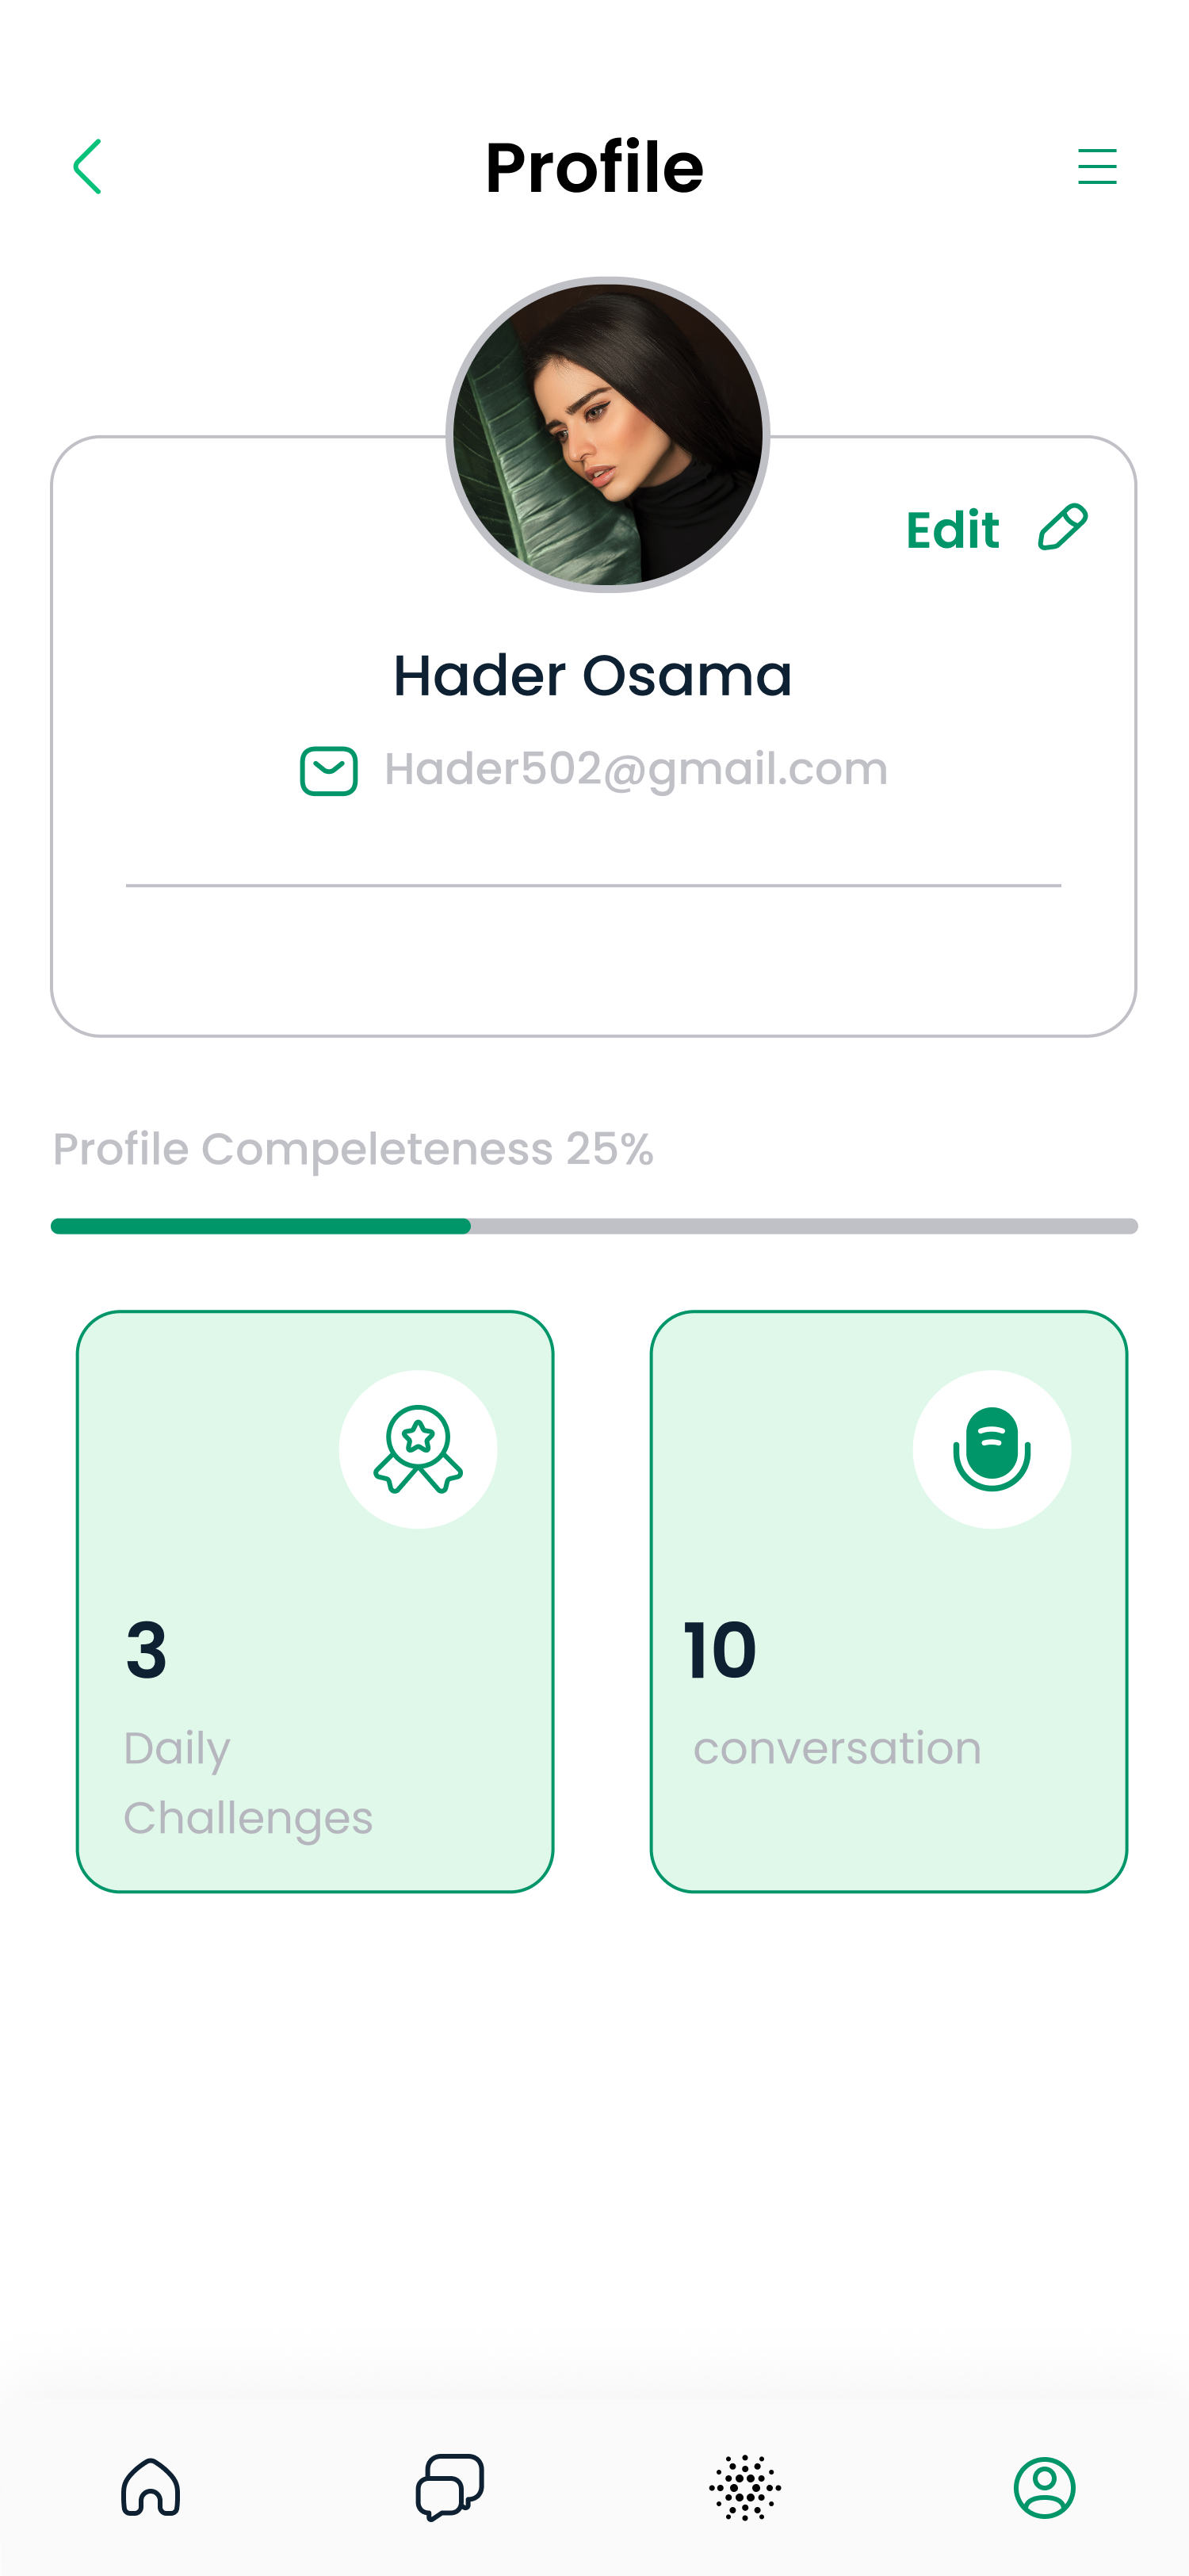
\includegraphics[width=\textwidth]{a13}}%
}%
    \end{minipage}
\end{figure}





 
% ------------------------------------------------------------------------------
% Reference list
% ------------------------------------------------------------------------------

% Specify the bibliography style
% \bibliographystyle{numeric}
\begingroup
\raggedright
\addcontentsline{toc}{chapter}{References}
    \renewcommand\bibname{References}
% \printbibliography
\endgroup
% ------------------------------------------------------------------------------
% Appendices
% ------------------------------------------------------------------------------
\include{appendix}

\end{document}

